% 第 5 章 Qt 图形应用
\renewcommand{\codeInset}{18bp}
本章介绍如何用 Qt 开发图形应用。在第 4 章「基于指针的图书馆管理系统」中，我们开发了抽象数据类型和一个图书馆管理系统，不过那些应用程序都是文本模式的。本章我们将研究三个用 Qt 图形库开发的图形应用：

\begin{itemize}
\item 时钟（clock）：我们开发一个模拟时钟，带有时针、分针和秒针，并用刻度线标记小时、分钟和秒。
\item 画图程序（drawing program）：一个用不同颜色绘制直线、矩形和椭圆的程序。
\item 编辑器（editor）：用户可以输入和编辑文本的程序。
\end{itemize}

我们还将学习 Qt 库的以下内容：

\begin{itemize}
\item 窗口与部件；
\item 菜单与工具栏；
\item 在窗口中绘制图形与书写文本；
\item 如何捕获鼠标和键盘事件。
\end{itemize}

\section{创建时钟应用程序}

本章以及下一章我们都将使用 Qt——一个面向对象的图形应用类库；同时我们使用的开发环境是 Qt Creator 而不是 Visual Studio，后者是一个集成开发环境。

\subsection{环境搭建}

在 Qt Creator 中创建新的图形工程时，我们在 File 菜单中选择 New File or Project 菜单项，此时会显示出 New File or Project 对话框窗口。我们选择 Qt Widgets Application，然后点击 Choose 按钮。

接着会显示 Introduction and Project Location 对话框。我们把工程命名为 Clock，放在合适的位置，然后点击 Next 按钮。在 Kit Selection 对话框中，我们选择最新版本的 Qt 库，然后点击 Next。在 Class Information 对话框中，我们把应用的基础类命名为 clock。通常，图形应用的窗口继承一个窗口类；不过这里要处理的是一个相对简单的应用，所以我们继承 Qt 的 QWidget 类——尽管部件（widget）通常指嵌在窗口中的较小图形对象。在 Qt Creator 中可以添加表单（form），但本章我们不使用该特性，因此取消勾选 Generate form 选项。

\begin{myNotic}{p171_i00}{Qt 中所有类名都以字母 Q 开头。}
\end{myNotic}

最后，在 Project Management 对话框中，我们直接接受默认值并点击 Finish，生成包含 Clock.h 和 Clock.cpp 文件的工程。

\subsection{Clock 类}

工程由 Clock.h、Clock.cpp 和 Main.cpp 文件组成。类定义与前面几章的类略有不同：我们用包含保护（include guard）把类定义包起来。也就是说，必须用预处理指令 \texttt{ifndef}、\texttt{define} 和 \texttt{endif} 把类定义包起来。预处理器执行文本替换。

\texttt{ifndef} 和 \texttt{endif} 指令的作用类似于 C++ 中的 \texttt{if} 语句。如果条件不成立，指令之间的代码就会被省略。这里，只有当 \texttt{CLOCK\_H} 宏尚未定义时才会包含这段代码；如果包含，下一行的 \texttt{define} 指令就会定义这个宏。这样，类定义在整个工程中只会被包含一次。此外，我们还在 Clock.h 头文件（而不是 Clock.cpp 定义文件）中包含系统头文件 QWidget 和 QTimer。

\medskip\noindent{\ttfamily\bfseries Clock.h}

\begin{codebox}
#ifndef CLOCK_H
#define CLOCK_H

#include <QWidget>
#include <QTimer>
\end{codebox}

由于 Clock 是 Qt QWidget 类的子类，必须包含 Q\_OBJECT 宏，它会引入 Qt 库中的某些代码。我们需要它来使用这里所示的 SIGNAL 和 SLOT 宏：

\begin{codebox}
class Clock : public QWidget {
  Q_OBJECT
\end{codebox}

构造函数接受一个指向父部件的指针，默认值为 \texttt{nullptr}：

\begin{codebox}
  public:
    Clock(QWidget* parentWidgetPtr = nullptr);
\end{codebox}

每当窗口需要重绘时，框架就会调用 paintEvent 方法。它接受一个指向 QPaintEvent 对象的指针作为参数，该参数可用于确定重绘应如何进行：

\begin{codebox}
    void paintEvent(QPaintEvent *eventPtr);
\end{codebox}

QTimer 是一个处理定时器的 Qt 系统类。我们将用它来移动时钟的指针：

\begin{codebox}
  private:
    QTimer m_timer;
  };

#endif // CLOCK_H
\end{codebox}

定义文件主要由处理时钟绘制的 paintEvent 方法组成。

\medskip\noindent{\ttfamily\bfseries Clock.cpp}

\begin{codebox}
#include <QtWidgets>
#include "Clock.h"
\end{codebox}

在构造函数中，我们调用基类 QWidget 的构造函数并传入 parentWidgetPtr 参数（它可以是 \texttt{nullptr}）：

\begin{codebox}
Clock::Clock(QWidget* parentWidgetPtr /* = nullptr */)
 :QWidget(parentWidgetPtr) {
\end{codebox}

我们把窗口标题设置为 Clock。在 Qt 中，字面文本总是用 tr 函数处理，它进而调用 Qt QCoreApplication 类中的 translate 方法，确保文本被转换为适合显示的形式。我们还将窗口大小调整为 1000 $\times$ 500 像素，这对大多数屏幕都合适：

\begin{codebox}
  setWindowTitle(tr("Clock"));
  resize(1000, 500);
\end{codebox}

我们需要一种把定时器与时钟部件连接起来的方法：定时器倒计时结束时，时钟应当被更新。为此，Qt 向我们提供了信号（signal）/槽（slot）机制。当定时器到达计时期限时，它会调用自身的 timeout 方法。我们用 connect 方法配合 SIGNAL 和 SLOT 宏，把对 timeout 的调用与 Qt QWidget 类中 update 方法的调用连接起来，后者更新时钟的绘制。SIGNAL 宏登记 timeout 调用将发出一个信号，SLOT 宏登记信号发出时应调用 update 方法，connect 方法则把信号与槽连接起来。这样，我们就在定时器的 timeout 与时钟的更新之间建立了一个连接：

\begin{codebox}
  m_timer.setParent(this);
  connect(&m_timer, SIGNAL(timeout()), this, SLOT(update()));
  m_timer.start(100);
}
\end{codebox}

每当窗口需要重绘时就会调用 paintEvent 方法。原因可能是外部因素，比如用户改变了窗口大小；也可能是对 QMainWindow 类 update 方法的调用，它最终会调用 paintEvent。

本例中我们不需要事件的任何信息，所以把 eventPtr 参数用注释括起来。width 和 height 方法给出窗口可绘制部分的宽度和高度（单位为像素）。我们调用 qMin 方法来决定窗口较短的那条边，并调用 QTime 类的 currentTime 方法来获取时钟的当前时间：

\begin{codebox}
void Clock::paintEvent(QPaintEvent* /* eventPtr */) {
  int side = qMin(width(), height());
  QTime time = QTime::currentTime();
\end{codebox}

QPainter 类可以看作一块绘图画布。我们首先把它初始化为合适的抗锯齿设置，然后调用 translate 和 scale 方法，把以像素为单位的物理尺寸变换为 200 $\times$ 200 单位的逻辑尺寸：

\begin{codebox}
  QPainter painter(this);
  painter.setRenderHint(QPainter::Antialiasing);
  painter.setRenderHint(QPainter::TextAntialiasing);
  painter.translate(width() / 2, height() / 2);
  painter.scale(side / 200.0, side / 200.0);
\end{codebox}

我们为分钟绘制 60 条刻度线。每第五条线要稍长一些，用来标记小时。对每一分钟，我们先画一条线，然后调用 Qt 的 rotate 方法把绘图旋转 6 度。这样，我们以 6 度为单位旋转 60 次，总共转过 360 度，即一整圈：

\begin{codebox}
  for (int second = 0; second <= 60; ++second) {
    if ((second % 5) == 0) {
      painter.drawLine(QPoint(0, 81), QPoint(0, 98));
    }
    else {
      painter.drawLine(QPoint(0, 90), QPoint(0, 98));
    }
\end{codebox}

一整圈是 360 度。每条线旋转 6 度，因为 360 除以 60 等于 6 度。旋转完毕后，把绘图恢复为初始设置：

\begin{codebox}
    painter.rotate(6);
  }
\end{codebox}

我们从 QTime 对象获取当前的时、分、秒和毫秒：

\begin{codebox}
  double hours = time.hour(), minutes = time.minute(),
         seconds = time.second(), milliseconds = time.msec();
\end{codebox}

我们把画笔颜色设为黑色，把背景色设为灰色：

\begin{codebox}
  painter.setPen(Qt::black);
  painter.setBrush(Qt::gray);
\end{codebox}

我们定义时针的端点。时针比分针和秒针稍粗稍短。我们定义构成时针端点的三个点。时针底座长 16 个单位，距原点 8 个单位，因此我们把底座两点的 x 坐标设为 8 和 $-8$，y 坐标设为 8。最后，把时针长度定义为 60 个单位。该值为负，以便与当前旋转方向一致：

\begin{codebox}
  { static const QPoint hourHand[3] =
        {QPoint(8, 8), QPoint(-8, 8), QPoint(0, -60)};
\end{codebox}

save 方法保存 QPainter 对象的当前设置，之后由 restore 方法恢复：

\begin{codebox}
    painter.save();
\end{codebox}

通过计算小时、分、秒和毫秒，我们求出时针的精确角度，然后旋转以设置时针。每小时对应 30 度，因为一圈有 12 个小时，360 度除以 12 等于 30 度：

\begin{codebox}
    double hour = hours + (minutes / 60.0) + (seconds / 3600.0) +
                  (milliseconds / 3600000.0);
    painter.rotate(30.0 * hour);
\end{codebox}

我们用时针的三个点调用 drawConvexPolygon 方法：

\begin{codebox}
    painter.drawConvexPolygon(hourHand, 3);
    painter.restore();
  }
\end{codebox}

我们以同样的方式绘制分针。它比时针稍细稍长。另一个区别是：小时有 12 个，分钟却有 60 个，因此每分钟对应 6 度——360 度除以 60 等于 6 度：

\begin{codebox}
  { static const QPoint minuteHand[3] =
        {QPoint(6, 8), QPoint(-6, 8), QPoint(0, -70)};
    painter.save();
\end{codebox}

计算当前分针角度时，我们使用分钟、秒和毫秒：

\begin{codebox}
    double minute = minutes + (seconds / 60.0) +
                    (milliseconds / 60000.0);
    painter.rotate(6.0 * minute);
    painter.drawConvexPolygon(minuteHand, 3);
    painter.restore();
  }
\end{codebox}

秒针的绘制与前面的分针几乎完全相同，唯一的区别是计算秒针角度时只使用秒和毫秒：

\begin{codebox}
  { static const QPoint secondHand[3] =
        {QPoint(4, 8), QPoint(-4, 8), QPoint(0, -80)};
    painter.save();
    double second = seconds + (milliseconds / 1000);
    painter.rotate(6.0 * second);
    painter.drawConvexPolygon(secondHand, 3);
    painter.restore();
  }
}
\end{codebox}

\subsection{main 函数}

在 main 函数中，我们初始化并启动 Qt 应用程序。main 函数可以接受参数 argc 和 argv，它们保存应用程序的命令行参数：argc 保存参数的个数，argv 数组保存参数本身。argv 的第一个元素总是可执行文件的路径，最后一个元素总是 \texttt{nullptr}。QApplication 类接受 argc 和 argv 并初始化 Qt 应用程序。我们创建一个 Clock 类的对象，并调用 show 使其可见。最后，调用 QApplication 对象的 exec。

\medskip\noindent{\ttfamily\bfseries Main.cpp}

\begin{codebox}
#include <QApplication>
#include "Clock.h"

int main(int argc, char *argv[]) {
  QApplication application(argc, argv);
  Clock Clock;
  Clock.show();
  return application.exec();
}
\end{codebox}

要执行应用程序，我们在项目上选择 Run 选项：

\begin{center}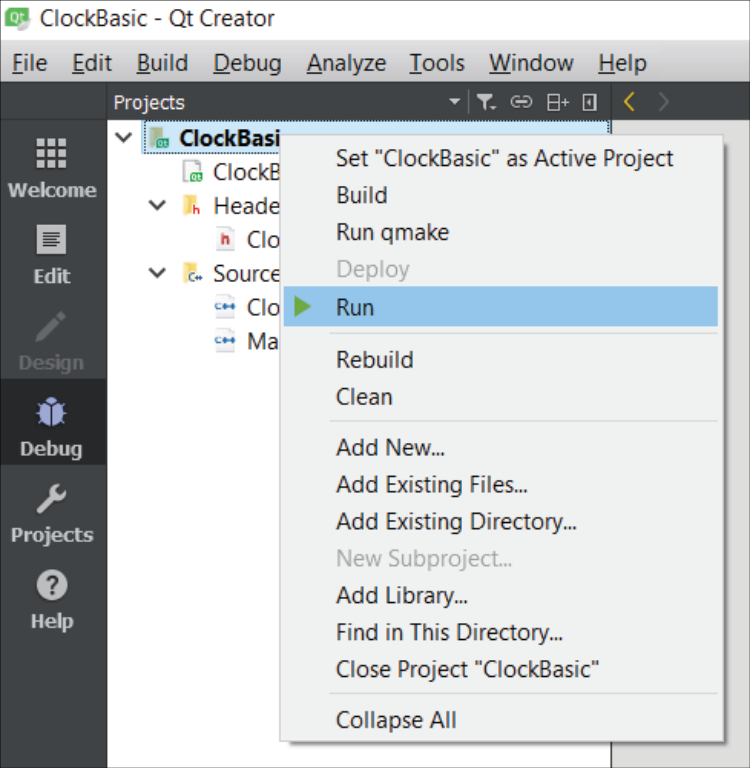
\includegraphics[width=0.7\textwidth]{images/p177_i03.png}\end{center}

程序的执行会一直持续到用户点击右上角的关闭按钮、关闭 Clock 窗口为止：

\begin{center}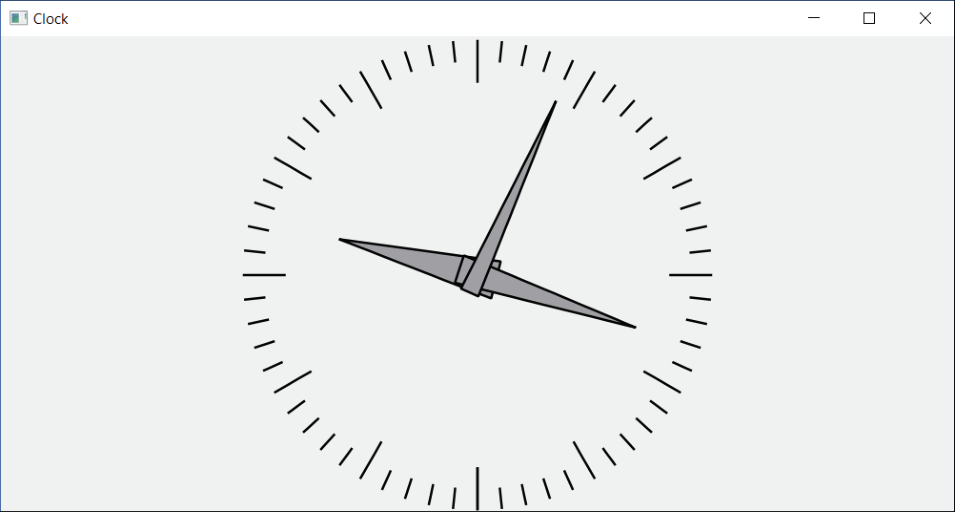
\includegraphics[width=0.9\textwidth]{images/p177_i05.png}\end{center}

\section{为窗口和部件搭建可复用的类}

图形应用中有窗口和部件。窗口通常是一个带边框的完整窗口，边框上有标题、菜单栏以及关闭窗口和调整窗口大小的按钮；而部件通常是嵌在窗口中的较小图形对象。在 Clock 工程中，我们只用了继承 QWidget 类的一个部件类。不过本节我们将离开 Clock 工程，研究更高级的同时包含窗口和部件的应用：窗口持有带菜单栏和工具栏的边框，而部件位于窗口中并负责图形内容。

本章接下来的各节中，我们将研究画图程序和编辑器。这些应用是典型的文档应用：我们打开和保存文档，还可以对文档元素进行剪切、复制、粘贴和删除。为了给窗口添加菜单和工具栏，我们需要继承 Qt 的两个类 QMainWindow 和 QWidget：QMainWindow 用于给窗口边框添加菜单和工具栏，QWidget 用于在窗口区域绘制图形。

为了在本章剩余部分以及下一章介绍的应用中复用文档代码，本节我们定义 MainWindow 和 DocumentWidget 类。这些类随后将被本章后面各节中的画图程序和编辑器使用。MainWindow 搭建带 File 和 Edit 菜单及工具栏的窗口，而 DocumentWidget 提供一个框架，为 New、Open、Save、SaveAs、Cut、Copy、Paste、Delete 和 Exit 菜单项搭建骨架代码。

本节我们不新建 Qt 工程，只编写 MainWindow 和 DocumentWidget 类——它们将作为本章后面画图程序和编辑器的基类，还有用于设置菜单和工具栏项的 LISTENER 宏。

\subsection{添加监听器}

监听器（listener）是用户选择菜单项或工具栏项时被调用的方法。LISTENER 宏向类添加一个监听器。

\medskip\noindent{\ttfamily\bfseries Listener.h}

\begin{codebox}
#ifndef LISTENER_H
#define LISTENER_H

#include <QObject>
\end{codebox}

由于 Qt 对菜单和工具栏的规定，Qt 框架响应用户操作而调用的监听器必须是函数而不是方法。

\begin{myNotic}{p179_i00}{方法属于类，而函数是自由独立的。}
\end{myNotic}

DEFINE\_LISTENER 宏同时定义一个友元函数和一个方法。Qt 框架调用该函数，函数再调用方法：

\begin{codebox}
#define DEFINE_LISTENER(BaseClass, Listener)
  friend bool Listener(QObject* baseObjectPtr) {
     return ((BaseClass*) baseObjectPtr)->Listener();
  }
  bool Listener()
\end{codebox}

LISTENER 宏定义为指向方法的指针：

\begin{codebox}
#define LISTENER(Listener) (&::Listener)
\end{codebox}

监听器方法接受一个 QObject 指针作为参数并返回布尔值：

\begin{codebox}
typedef bool (*Listener)(QObject*);
#endif // LISTENER_H
\end{codebox}

\subsection{基窗口类}

MainWindow 类搭建一个带 File 和 Edit 菜单及工具栏的文档窗口。它还提供 addAction 方法，供子类添加应用专属的菜单和工具栏。

\medskip\noindent{\ttfamily\bfseries MainWindow.h}

\begin{codebox}
#ifndef MAINWINDOW_H
#define MAINWINDOW_H

#include <QMainWindow>
#include <QActionGroup>
#include <QPair>
#include <QMap>

#include "Listener.h"
#include "DocumentWidget.h"

class MainWindow : public QMainWindow {
  Q_OBJECT

  public:
    MainWindow(QWidget* parentWidgetPtr = nullptr);
    ~MainWindow();

  protected:
    void addFileMenu();
    void addEditMenu();
\end{codebox}

addAction 方法添加一个菜单项，可带快捷键、工具栏图标，以及用于给菜单项标注复选框或单选按钮的监听器：

\begin{codebox}
  protected:
    void addAction(QMenu* menuPtr, QString text,
                   const char* onSelectPtr,
                   QKeySequence acceleratorKey = 0,
                   QString iconName = QString(),
                   QToolBar* toolBarPtr = nullptr,
                   QString statusTip = QString(),
                   Listener enableListener = nullptr,
                   Listener checkListener = nullptr,
                   QActionGroup* groupPtr = nullptr);
\end{codebox}

我们用 DEFINE\_LISTENER 宏添加监听器，用于决定菜单项是否应处于启用状态。监听器在菜单项应启用时返回 true。DocumentWidget 是 Qt 类 QWidget 的子类，我们将在下一小节定义它。借助 DEFINE\_LISTENER 宏，我们给 MainWindow 类添加 isSaveEnabled、isCutEnabled、isCopyEnabled、isPasteEnabled 和 isDeleteEnabled 方法。当用户选择菜单项时会调用它们：

\begin{codebox}
    DEFINE_LISTENER(DocumentWidget, isSaveEnabled);
    DEFINE_LISTENER(DocumentWidget, isCutEnabled);
    DEFINE_LISTENER(DocumentWidget, isCopyEnabled);
    DEFINE_LISTENER(DocumentWidget, isPasteEnabled);
    DEFINE_LISTENER(DocumentWidget, isDeleteEnabled);
\end{codebox}

onMenuShow 方法在菜单变为可见之前被调用；它调用菜单中各菜单项的监听器，以决定菜单项应被禁用，还是标注复选框或单选按钮。框架也会调用它来禁用工具栏图标：

\begin{codebox}
  public slots:
    void onMenuShow();
\end{codebox}

m\_enableMap 和 m\_checkMap 字段保存菜单项监听器的映射。前面的 onMenuShow 方法用它们来决定禁用菜单项，还是标注复选框或单选按钮：

\begin{codebox}
  private:
    QMap<QAction*,QPair<QObject*,Listener>> m_enableMap,
                                            m_checkMap;
  };

#endif // MAINWINDOW_H
\end{codebox}

\medskip\noindent{\ttfamily\bfseries MainWindow.cpp}

\begin{codebox}
#include "MainWindow.h"
#include <QtWidgets>
\end{codebox}

构造函数调用 Qt QMainWindow 类的构造函数，参数是父部件指针：

\begin{codebox}
MainWindow::MainWindow(QWidget* parentWidgetPtr /*= nullptr*/)
 :QMainWindow(parentWidgetPtr) {
}
\end{codebox}

菜单项添加时会连接到一个动作（action）。析构函数释放菜单栏的所有动作：

\begin{codebox}
MainWindow::~MainWindow() {
  for (QAction* actionPtr : menuBar()->actions()) {
    delete actionPtr;
  }
}
\end{codebox}

addFileMenu 方法把标准 File 菜单添加到菜单栏；menuBar 是一个 Qt 方法，返回窗口菜单栏的指针：

\begin{codebox}
void MainWindow::addFileMenu() {
  QMenu* fileMenuPtr = menuBar()->addMenu(tr("&File"));
\end{codebox}

下面的代码片段与 connect 方法类似，把菜单项与 onMenuShow 方法连接起来。Qt 宏 SIGNAL 和 SLOT 确保在菜单变为可见之前调用 onMenuShow。onMenuShow 方法在菜单可见之前设置菜单中每一项的启用、复选框和单选按钮状态；它还设置工具栏图标的启用状态。aboutToShow 方法在每个菜单可见之前被调用，以便启用或禁用菜单项，并可能给它们标注复选框或单选按钮：

\begin{codebox}
  connect(fileMenuPtr, SIGNAL(aboutToShow()), this,
          SLOT(onMenuShow()));
\end{codebox}

Qt 的 addToolBar 方法向窗口边框添加一个工具栏。在这里调用 addAction 时，菜单项会被添加到菜单中；如果存在对应的工具栏，也会添加到工具栏：

\begin{codebox}
  QToolBar *fileToolBarPtr = addToolBar(tr("File"));
\end{codebox}

addAction 方法添加 New、Open、Save、SaveAs 和 Exit 菜单项。它接受以下参数：

\begin{itemize}
\item 菜单项所属菜单的指针。
\item 菜单项文本。文本前的和号（\texttt{\&}）（如 \texttt{\&New}）表示紧随其后的字母（N）将带下划线，用户可按 Alt-N 选择该项。
\item 快捷键信息。QKeySequence 是保存快捷键组合的 Qt 枚举。QKeySequence::New 表示用户可按 Ctrl-N 选择该项，菜单项文本后还会附加上 Ctrl+N。
\item 图标文件的名称（new）。该文件的图标显示在菜单项文本左侧和工具栏上。图标文件本身在 Qt Creator 中添加到工程。
\item 工具栏的指针；如果菜单项不连接工具栏，则为 \texttt{nullptr}。
\item 用户把鼠标悬停在工具栏项上时显示的文本。如果菜单项不连接工具栏，则被忽略。
\item 监听器（默认 \texttt{nullptr}），在菜单和工具栏变为可见之前调用，决定该项是启用，还是标注复选框或单选按钮。
\end{itemize}

\begin{codebox}
  addAction(fileMenuPtr, tr("&New"), SLOT(onNew()),
            QKeySequence::New, tr("new"), fileToolBarPtr,
            tr("Create a new file"));

  addAction(fileMenuPtr, tr("&Open"), SLOT(onOpen()),
            QKeySequence::Open, tr("open"), fileToolBarPtr,
            tr("Open an existing file"));
\end{codebox}

当文档自上次保存后没有更改时，文档无需保存，Save 菜单项应禁用。因此我们添加一个额外的参数，指明应调用 isSaveEnabled 方法来启用或禁用菜单项和工具栏图标：

\begin{codebox}
  addAction(fileMenuPtr, tr("&Save"), SLOT(onSave()),
            QKeySequence::Save, tr("save"), fileToolBarPtr,
            tr("Save the document to disk"),
            LISTENER(isSaveEnabled));
\end{codebox}

SaveAs 菜单项没有按键序列，也没有工具栏项。因此图标文件名和工具栏文本是默认的 QString 对象，工具栏指针为 \texttt{nullptr}：

\begin{codebox}
  addAction(fileMenuPtr, tr("Save &As"), SLOT(onSaveAs()),
            0, QString(), nullptr, QString(),
            LISTENER(isSaveEnabled));
\end{codebox}

addSeparator 方法在两个菜单项之间添加一条水平分隔线：

\begin{codebox}
  fileMenuPtr->addSeparator();
  addAction(fileMenuPtr, tr("E&xit"),
            SLOT(onExit()), QKeySequence::Quit);
}
\end{codebox}

addEditMenu 方法以与前面 File 菜单相同的方式把 Edit 菜单添加到窗口菜单栏：

\begin{codebox}
void MainWindow::addEditMenu() {
  QMenu* editMenuPtr = menuBar()->addMenu(tr("&Edit"));
  QToolBar* editToolBarPtr = addToolBar(tr("Edit"));
  connect(editMenuPtr, SIGNAL(aboutToShow()),
          this, SLOT(onMenuShow()));

  addAction(editMenuPtr, tr("&Cut"), SLOT(onCut()),
            QKeySequence::Cut, tr("cut"), editToolBarPtr,
        tr("Cut the current selection's contents to the clipboard"),
            LISTENER(isCutEnabled));

  addAction(editMenuPtr, tr("&Copy"), SLOT(onCopy()),
            QKeySequence::Copy, tr("copy"), editToolBarPtr,
         tr("Copy the current selection's contents to the clipboard"),
            LISTENER(isCopyEnabled));

  addAction(editMenuPtr, tr("&Paste"),
            SLOT(onPaste()),
            QKeySequence::Paste, tr("paste"), editToolBarPtr,
        tr("Paste the current selection's contents to the clipboard"),
            LISTENER(isPasteEnabled));

  editMenuPtr->addSeparator();
  addAction(editMenuPtr, tr("&Delete"), SLOT(onDelete()),
            QKeySequence::Delete, tr("delete"), editToolBarPtr,
            tr("Delete the current selection"),
            LISTENER(isDeleteEnabled));
}
\end{codebox}

addAction 方法向菜单栏添加菜单项并向工具栏添加工具栏图标，还把菜单项与用户选择该项时被调用的 onSelectPtr 方法，以及启用该项、标注复选框或单选按钮的方法连接起来。除非快捷键为零，否则会为动作添加快捷键。groupPtr 参数定义菜单项是否属于一个组。如果 checkListener 不是 \texttt{nullptr}，那么当 groupPtr 为 \texttt{nullptr} 时菜单项标注复选框，否则标注单选按钮。对于单选按钮，同一时刻每组只有一个会被选中：

\begin{codebox}
void MainWindow::addAction(QMenu* menuPtr, QString itemText,
                           const char* onSelectPtr,
                           QKeySequence acceleratorKey /* = 0 */,
                           QString iconName /*= QString()*/,
                           QToolBar* toolBarPtr /*= nullptr*/,
                           QString statusTip /*= QString()*/,
                           Listener enableListener /*= nullptr*/,
                           Listener checkListener /*= nullptr*/,
                           QActionGroup* groupPtr /*= nullptr*/) {
  QAction* actionPtr;
\end{codebox}

如果 iconName 非空，我们从工程资源中的文件加载图标，然后创建带图标的新 QAction 对象：

\begin{codebox}
  if (!iconName.isEmpty()) {
    const QIcon icon = QIcon::fromTheme("document-" + iconName,
                       QIcon(":/images/" + iconName + ".png"));
    actionPtr = new QAction(icon, itemText, this);
  }
\end{codebox}

如果 iconName 为空，我们创建不带图标的新 QAction 对象：

\begin{codebox}
  else {
    actionPtr = new QAction(itemText, this);
  }
\end{codebox}

我们把菜单项连接到选择方法。当用户选择菜单项或点击工具栏图标时，会调用 onSelectPtr：

\begin{codebox}
  connect(actionPtr, SIGNAL(triggered()),
          centralWidget(), onSelectPtr);
\end{codebox}

如果快捷键不为零，我们把它加到动作指针上：

\begin{codebox}
  if (acceleratorKey != 0) {
    actionPtr->setShortcut(acceleratorKey);
  }
\end{codebox}

最后，我们把动作指针加到菜单指针上，以便菜单处理用户的选择：

\begin{codebox}
  menuPtr->addAction(actionPtr);
\end{codebox}

如果 toolBarPtr 不是 \texttt{nullptr}，我们把动作添加到窗口的工具栏：

\begin{codebox}
  if (toolBarPtr != nullptr) {
    toolBarPtr->addAction(actionPtr);
  }
\end{codebox}

如果状态提示非空，我们把它添加到工具栏的工具提示（tooltip）和状态提示中：

\begin{codebox}
  if (!statusTip.isEmpty()) {
      actionPtr->setToolTip(statusTip);
      actionPtr->setStatusTip(statusTip);
  }
\end{codebox}

如果启用监听器不为空，我们向 m\_enableMap 添加一个由窗口中央部件指针和监听器组成的对，并调用该监听器来初始化菜单项和工具栏图标的启用状态：

\begin{codebox}
  if (enableListener != nullptr) {
    QWidget* widgetPtr = centralWidget();
    m_enableMap[actionPtr] =
      QPair<QObject*,Listener>(widgetPtr, enableListener);
    actionPtr->setEnabled(enableListener(widgetPtr));
  }
\end{codebox}

同样，如果复选监听器不为空，我们向 m\_checkMap 添加窗口中央部件指针和监听器。m\_enableMap 和 m\_checkMap 都由 onMenuShow 使用，方式如下。我们还调用该监听器来初始化菜单项的复选状态（工具栏图标不复选）：

\begin{codebox}
  if (checkListener != nullptr) {
    actionPtr->setCheckable(true);
    QWidget* widgetPtr = centralWidget();
    m_checkMap[actionPtr] =
      QPair<QObject*,Listener>(widgetPtr, checkListener);
    actionPtr->setChecked(checkListener(widgetPtr));
  }
\end{codebox}

最后，如果组指针不为空，我们把动作加入该组。这样，菜单项将标注单选按钮而不是复选框。框架还会跟踪各组，确保同一时刻每组只有一个单选按钮被选中：

\begin{codebox}
  if (groupPtr != nullptr) {
    groupPtr->addAction(actionPtr);
  }
}
\end{codebox}

onMenuShow 方法在菜单或工具栏图标变为可见之前被调用。它确保每个菜单项被启用或禁用，并确保菜单项标注复选框或单选按钮。

我们首先遍历启用映射。对映射中的每一项，我们查找部件和启用函数，调用该函数得到 true 或 false，并用结果通过在动作对象指针上调用 setEnabled 来启用或禁用菜单项：

\begin{codebox}
void MainWindow::onMenuShow() {
  for (QMap<QAction*,QPair<QObject*,Listener>>::iterator i =
       m_enableMap.begin(); i != m_enableMap.end(); ++i) {
    QAction* actionPtr = i.key();
    QPair<QObject*,Listener> pair = i.value();
    QObject* baseObjectPtr = pair.first;
    Listener enableFunction = pair.second;
    actionPtr->setEnabled(enableFunction(baseObjectPtr));
  }
\end{codebox}

同样，我们遍历复选映射。对每一项，我们查找部件和复选函数，调用该函数并用结果通过在动作对象指针上调用 setCheckable 和 setChecked 来复选菜单项。如果菜单项属于某个组，Qt 框架确保它标注单选按钮；否则标注复选框：

\begin{codebox}
  for (QMap<QAction*,QPair<QObject*,Listener>>::iterator i =
       m_checkMap.begin(); i != m_checkMap.end(); ++i) {
    QAction* actionPtr = i.key();
    QPair<QObject*,Listener> pair = i.value();
    QObject* baseObjectPtr = pair.first;
    Listener checkFunction = pair.second;
    actionPtr->setCheckable(true);
    actionPtr->setChecked(checkFunction(baseObjectPtr));
  }
}
\end{codebox}

\subsection{基部件类}

DocumentWidget 是处理文档的应用的骨架框架。它处理文档的加载与保存，并提供供子类重写的方法，对应 Cut、Copy、Paste 和 Delete 菜单项。

前面的 MainWindow 类处理窗口边框及其菜单和工具栏，而 DocumentWidget 类负责绘制窗口的内容。思路是：MainWindow 的子类创建一个 DocumentWidget 子类的对象，并把它放到窗口中央。参见后面各节中 DrawingWindow 和 EditorWindow 的构造函数。

\medskip\noindent{\ttfamily\bfseries DocumentWidget.h}

\begin{codebox}
#ifndef DOCUMENTWIDGET_H
#define DOCUMENTWIDGET_H

#include "Listener.h"
#include <QWidget>
#include <QtWidgets>
#include <FStream>
using namespace std;

class DocumentWidget : public QWidget {
  Q_OBJECT
\end{codebox}

构造函数接受应用名称（显示在窗口顶部横幅上）、用标准文件对话框加载和保存文档时使用的文件名掩码，以及指向潜在父部件（通常是外层主窗口）的指针：

\begin{codebox}
  public:
    DocumentWidget(const QString& name, const QString& fileMask,
                   QWidget* parentWidgetPtr);
    ~DocumentWidget();
\end{codebox}

setFilePath 方法设置当前文档的路径。路径显示在窗口顶部横幅上，并作为标准加载和保存对话框中的默认路径：

\begin{codebox}
  protected:
    void setFilePath(QString filePath);
\end{codebox}

文档更改后，modified 标志（有时称为 dirty 标志）被置位。这会使窗口顶部横幅上的文件路径旁出现一个星号（*），并启用 Save 和 SaveAs 菜单项：

\begin{codebox}
  public:
    void setModifiedFlag(bool flag);
\end{codebox}

setMainWindowTitle 方法是一个辅助方法，用于拼出窗口的标题。它由文件路径以及一个可能的星号（*）组成，星号表示 modified 标志已置位：

\begin{codebox}
  private:
    void setMainWindowTitle();
\end{codebox}

closeEvent 方法从 QWidget 重写而来，在用户关闭窗口时被调用。通过设置 eventPtr 参数的字段，可以阻止关闭。例如，如果文档尚未保存，可以询问用户是要保存文档，还是取消关闭窗口：

\begin{codebox}
  public:
    virtual void closeEvent(QCloseEvent* eventPtr);
\end{codebox}

isClearOk 方法是一个辅助方法，当用户试图在未保存文档的情况下关闭窗口或退出应用时，它会显示一个消息框：

\begin{codebox}
  private:
    bool isClearOk(QString title);
\end{codebox}

用户选择菜单项或点击工具栏图标时，框架会调用下列方法。为此，我们把方法标记为槽（slot），这是 connect 调用中 SLOT 宏所必需的：

\begin{codebox}
  public slots:
    virtual void onNew();
    virtual void onOpen();
    virtual bool onSave();
    virtual bool onSaveAs();
    virtual void onExit();
\end{codebox}

文档未更改时无需保存。此时应禁用 Save 和 SaveAs 菜单项及工具栏图标。onMenuShow 在 File 菜单可见之前调用 isSaveEnabled 方法。只有当文档已更改且需要保存时，它才返回 true：

\begin{codebox}
    virtual bool isSaveEnabled();
\end{codebox}

tryWriteFile 方法是一个辅助方法，它尝试写文件。如果失败，消息框会显示一条错误消息：

\begin{codebox}
    private:
        bool tryWriteFile(QString filePath);
\end{codebox}

下面的方法是打算被子类重写的虚方法，在用户选择 New、Save、SaveAs 和 Open 菜单项时被调用：

\begin{codebox}
  protected:
    virtual void newDocument() = 0;
    virtual bool writeFile(const QString& filePath) = 0;
    virtual bool readFile(const QString& filePath) = 0;
\end{codebox}

下面的方法在 Edit 菜单可见之前被调用，它们决定 Cut、Copy、Paste 和 Delete 菜单项是否应启用：

\begin{codebox}
  public:
    virtual bool isCutEnabled();
    virtual bool isCopyEnabled();
    virtual bool isPasteEnabled();
    virtual bool isDeleteEnabled();
\end{codebox}

下面的方法在用户选择 Cut、Copy、Paste 和 Delete 菜单项或工具栏图标时被调用：

\begin{codebox}
  public slots:
    virtual void onCut();
    virtual void onCopy();
    virtual void onPaste();
    virtual void onDelete();
\end{codebox}

m\_applicationName 字段保存应用的名称，而不是文档的名称。后面各节中名称将是 Drawing 和 Editor。m\_fileMask 字段保存用标准对话框加载和保存文档时使用的掩码。举例来说，假设文档以 \texttt{.abc} 结尾，那么掩码可以是 Abc files (*.abc)。m\_filePath 字段保存当前文档的路径。当文档是新的且尚未保存时，该字段保存空字符串。最后，m\_modifiedFlag 在文档已修改、需要在应用退出前保存时为 true：

\begin{codebox}
  private:
    QString m_applicationName, m_fileMask, m_filePath;
    bool m_modifiedFlag = false;
  };
\end{codebox}

最后还有一些重载的辅助运算符。加法和减法运算符把一个点与一个尺寸相加减，把一个矩形与一个尺寸相加减：

\begin{codebox}
QPoint& operator+=(QPoint& point, const QSize& size);
QPoint& operator-=(QPoint& point, const QSize& size);

QRect& operator+=(QRect& rect, int size);
QRect& operator-=(QRect& rect, int size);
\end{codebox}

writePoint 和 readPoint 方法从输入流写入和读取一个点：

\begin{codebox}
void writePoint(ofstream& outStream, const QPoint& point);
void readPoint(ifstream& inStream, QPoint& point);
\end{codebox}

writeColor 和 readColor 方法从输入流写入和读取一个颜色：

\begin{codebox}
void writeColor(ofstream& outStream, const QColor& color);
void readColor(ifstream& inStream, QColor& color);
\end{codebox}

makeRect 方法创建一个以 point 为中心、以 size 为大小的矩形：

\begin{codebox}
QRect makeRect(const QPoint& centerPoint, int halfSide);
#endif // DOCUMENTWIDGET_H
\end{codebox}

\medskip\noindent{\ttfamily\bfseries DocumentWidget.cpp}

\begin{codebox}
#include <QtWidgets>
#include <QMessageBox>

#include "MainWindow.h"
#include "DocumentWidget.h"
\end{codebox}

构造函数设置应用名称、保存和加载标准对话框的文件掩码，以及指向外层父部件（通常是外层主窗口）的指针：

\begin{codebox}
DocumentWidget::DocumentWidget(const QString& name,
                const QString& fileMask, QWidget* parentWidgetPtr)
 :m_applicationName(name),
  m_fileMask(fileMask),
  QWidget(parentWidgetPtr) {
  setMainWindowTitle();
}
\end{codebox}

析构函数什么也不做，包含它只是为了完整起见：

\begin{codebox}
DocumentWidget::~DocumentWidget() {
  // Empty.
}
\end{codebox}

setFilePath 方法调用 setMainWindowTitle 来更新窗口顶部横幅上的文本：

\begin{codebox}
void DocumentWidget::setFilePath(QString filePath) {
  m_filePath = filePath;
  setMainWindowTitle();
}
\end{codebox}

setModifiedFlag 方法同样调用 setMainWindowTitle 来更新窗口顶部横幅上的文本。此外，它还调用父部件的 onMenuShow 来更新工具栏的图标：

\begin{codebox}
void DocumentWidget::setModifiedFlag(bool modifiedFlag) {
  m_modifiedFlag = modifiedFlag;
  setMainWindowTitle();
  ((MainWindow*) parentWidget())->onMenuShow();
}
\end{codebox}

工具栏顶部横幅上显示的标题是应用名称、文档文件路径（如果非空），以及文档已修改但尚未保存时的一个星号：

\begin{codebox}
void DocumentWidget::setMainWindowTitle() {
  QString title= m_applicationName +
          (m_filePath.isEmpty() ? "" : (" [" + m_filePath + "]"))+
          (m_modifiedFlag ? " *" : "");
  this->parentWidget()->setWindowTitle(title);
}
\end{codebox}

isClearOk 方法在文档已修改但尚未保存时显示一个消息框。用户可以选择以下按钮之一：

\begin{itemize}
\item \textbf{Yes}：保存文档，应用退出。不过如果保存失败，会显示一条错误消息，应用不会退出。
\item \textbf{No}：应用不保存文档直接退出。
\item \textbf{Cancel}：取消应用的关闭。文档不保存。
\end{itemize}

\begin{codebox}
bool DocumentWidget::isClearOk(QString title) {
  if (m_modifiedFlag) {
    QMessageBox messageBox(QMessageBox::Warning,
                           title, QString());
    messageBox.setText(tr("The document has been modified."));
    messageBox.setInformativeText(
               tr("Do you want to save your changes?"));
    messageBox.setStandardButtons(QMessageBox::Yes |
                          QMessageBox::No | QMessageBox::Cancel);
    messageBox.setDefaultButton(QMessageBox::Yes);

    switch (messageBox.exec()) {
      case QMessageBox::Yes:
        return onSave();

      case QMessageBox::No:
        return true;

      case QMessageBox::Cancel:
        return false;
    }
  }

  return true;
}
\end{codebox}

如果文档被清除，则调用 newDocument——该方法打算被子类重写以执行应用专属的初始化。此外，modified 标志和文件路径被清除。最后，调用 Qt 的 update 方法强制重绘窗口的内容：

\begin{codebox}
void DocumentWidget::onNew() {
  if (isClearOk(tr("New File"))) {
    newDocument();
    setModifiedFlag(false);
    setFilePath(QString());
    update();
  }
}
\end{codebox}

如果文档被清除，onOpen 用标准打开对话框获得文档的文件路径：

\begin{codebox}
void DocumentWidget::onOpen() {
  if (isClearOk(tr("Open File"))) {
    QString file =
      QFileDialog::getOpenFileName(this, tr("Open File"),
                   tr("C:\Users\Stefan\Documents\"
                      "A A_Cpp_By_Example\Draw"),
              m_fileMask + tr(";;Text files (*.txt)"));
\end{codebox}

如果文件成功读取，则清除 modified 标志、设置文件路径，并调用 update 强制重绘窗口：

\begin{codebox}
    if (!file.isEmpty()) {
      if (readFile(file)) {
        setModifiedFlag(false);
        setFilePath(file);
        update();
      }
\end{codebox}

如果读取不成功，则显示一条带错误消息的消息框：

\begin{codebox}
      else {
        QMessageBox messageBox;
        messageBox.setIcon(QMessageBox::Critical);
        messageBox.setText(tr("Read File"));
        messageBox.setInformativeText(tr("Could not read \"") +
                                      m_filePath  + tr("\""));
        messageBox.setStandardButtons(QMessageBox::Ok);
        messageBox.setDefaultButton(QMessageBox::Ok);
        messageBox.exec();
      }
    }
  }
}
\end{codebox}

isSaveEnabled 方法只返回 m\_modifiedFlag 的值。不过，我们需要这个方法监听器才能工作：

\begin{codebox}
bool DocumentWidget::isSaveEnabled() {
  return m_modifiedFlag;
}
\end{codebox}

用户选择 Save 或 SaveAs 菜单项或工具栏图标时调用 onSave 方法。如果文档已经命名，我们就直接尝试写文件；如果尚未命名，则调用 onSaveAs，为用户显示标准的保存对话框：

\begin{codebox}
bool DocumentWidget::onSave() {
  if (!m_filePath.isEmpty()) {
    return tryWriteFile(m_filePath);
  }
  else {
    return onSaveAs();
  }
}
\end{codebox}

用户选择 SaveAs 菜单项（该项没有工具栏图标）时调用 onSaveAs 方法。它打开标准打开对话框并尝试写文件。如果写入不成功，则返回 false。原因是：只有写入成功时 isClearOk 才会关闭窗口：

\begin{codebox}
bool DocumentWidget::onSaveAs() {
  QString filePath =
          QFileDialog::getSaveFileName(this, tr("Save File"),
               tr("C:\Users\Stefan\Documents\"
                  "A A_Cpp_By_Example\Draw"),
            m_fileMask + tr(";;Text files (*.txt)"));

  if (!filePath.isEmpty()) {
    return tryWriteFile(filePath);
  }
  else {
    return false;
  }
}
\end{codebox}

tryWriteFile 方法通过调用 write——该方法打算被子类重写——尝试写文件。如果成功，设置 modified 标志和文件路径。如果文件写入不成功，则显示一条带错误消息的消息框：

\begin{codebox}
bool DocumentWidget::tryWriteFile(QString filePath) {
  if (writeFile(filePath)) {
    setModifiedFlag(false);
    setFilePath(filePath);
    return true;
  }
  else {
    QMessageBox messageBox;
    messageBox.setIcon(QMessageBox::Critical);
    messageBox.setText(tr("Write File"));
    messageBox.setInformativeText(tr("Could not write \"") +
                                  filePath  + tr("\""));
    messageBox.setStandardButtons(QMessageBox::Ok);
    messageBox.setDefaultButton(QMessageBox::Ok);
    messageBox.exec();
    return false;
  }
}
\end{codebox}

用户选择 Exit 菜单项时调用 onExit 方法。它检查是否可以关闭窗口，如果可以则退出应用：

\begin{codebox}
void DocumentWidget::onExit() {
  if (isClearOk(tr("Exit"))) {
    qApp->exit(0);
  }
}
\end{codebox}

isCutEnabled 和 isDeleteEnabled 的默认行为是调用 isCopyEnabled，因为它们通常在相同的条件下启用：

\begin{codebox}
bool DocumentWidget::isCutEnabled() {
  return isCopyEnabled();
}

bool DocumentWidget::isDeleteEnabled() {
  return isCopyEnabled();
}
\end{codebox}

onCut 的默认行为是直接调用 onCopy 和 onDelete：

\begin{codebox}
void DocumentWidget::onCut() {
  onCopy();
  onDelete();
}
\end{codebox}

剪切和复制方法组中其余方法的默认行为是返回 false 并什么也不做，这会让菜单项保持禁用状态，除非子类重写这些方法：

\begin{codebox}
bool DocumentWidget::isCopyEnabled() {
  return false;
}

void DocumentWidget::onCopy() {
  // Empty.
}

bool DocumentWidget::isPasteEnabled() {
  return false;
}

void DocumentWidget::onPaste() {
  // Empty.
}

void DocumentWidget::onDelete() {
  // Empty.
}
\end{codebox}

最后，用户试图关闭窗口时调用 closeEvent。如果窗口可以清除，就在 eventPtr 上调用 accept——这会关闭窗口——并对全局对象 qApp 调用 exit，使应用退出：

\begin{codebox}
void DocumentWidget::closeEvent(QCloseEvent* eventPtr) {
  if (isClearOk(tr("Close Window"))) {
    eventPtr->accept();
    qApp->exit(0);
  }
\end{codebox}

如果窗口不能清除，就在 eventPtr 上调用 ignore，窗口保持打开（应用继续运行）：

\begin{codebox}
  else {
    eventPtr->ignore();
  }
}
\end{codebox}

此外，还有一组用于处理点、尺寸、矩形和颜色的辅助函数。下面的运算符把一个点与一个尺寸相加减，并返回得到的点：

\begin{codebox}
QPoint& operator+=(QPoint& point, const QSize& size) {
  point.setX(point.x() + size.width());
  point.setY(point.y() + size.height());
  return point;
}

QPoint& operator-=(QPoint& point, const QSize& size) {
  point.setX(point.x() - size.width());
  point.setY(point.y() - size.height());
  return point;
}
\end{codebox}

下面的运算符把一个整数与矩形相加减，并返回得到的矩形。加法运算符把矩形的大小向每个方向扩大，减法运算符把矩形向每个方向缩小：

\begin{codebox}
QRect& operator+=(QRect& rect, int size) {
  rect.setLeft(rect.left() - size);
  rect.setTop(rect.top() - size);
  rect.setWidth(rect.width() + size);
  rect.setHeight(rect.height() + size);
  return rect;
}

QRect& operator-=(QRect& rect, int size) {
  rect.setLeft(rect.left() + size);
  rect.setTop(rect.top() + size);
  rect.setWidth(rect.width() - size);
  rect.setHeight(rect.height() - size);
  return rect;
}
\end{codebox}

writePoint 和 readPoint 函数从文件写入和读取一个点。它们分别写入和读取 x 和 y 坐标：

\begin{codebox}
void writePoint(ofstream& outStream, const QPoint& point) {
  int x = point.x(), y = point.y();
  outStream.write((char*) &x, sizeof x);
  outStream.write((char*) &y, sizeof y);
}

void readPoint(ifstream& inStream, QPoint& point) {
  int x, y;
  inStream.read((char*) &x, sizeof x);
  inStream.read((char*) &y, sizeof y);
  point = QPoint(x, y);
}
\end{codebox}

writeColor 和 readColor 函数从文件写入和读取一个颜色。一个颜色由红、绿、蓝三个分量组成，每个分量是 0 到 255（含两端）之间的整数值。这两个函数从文件流写入和读取各分量：

\begin{codebox}
void writeColor(ofstream& outStream, const QColor& color) {
  int red = color.red(), green = color.green(),
  blue = color.blue();
  outStream.write((char*) &red, sizeof red);
  outStream.write((char*) &green, sizeof green);
  outStream.write((char*) &blue, sizeof blue);
}

void readColor(ifstream& inStream, QColor& color) {
  int red, green, blue;
  inStream.read((char*) &red, sizeof red);
  inStream.read((char*) &green, sizeof green);
  inStream.read((char*) &blue, sizeof blue);
\end{codebox}

读取完各分量后，我们创建一个 QColor 对象并把它赋给 color 参数：

\begin{codebox}
  color = QColor(red, green, blue);
}
\end{codebox}

makeRect 函数创建一个以该点为中心的矩形：

\begin{codebox}
QRect makeRect(const QPoint& centerPoint, int halfSide) {
  return QRect(centerPoint.x() - halfSide,
               centerPoint.y() - halfSide,
               2 * halfSide, 2 * halfSide);
}
\end{codebox}

\section{构建画图程序}

现在我们开始一个新工程，利用上一节的主窗口类和文档部件类——也就是画图程序。本章我们先实现一个基础版本，下一章再继续构建更高级的版本。用本章的画图程序，我们可以用不同颜色绘制直线、矩形和椭圆，还可以保存和加载我们的绘图。注意，本工程中的窗口类和部件类继承自上一节的 MainWindow 和 DocumentWidget 类。

\subsection{Figure 基类}

应用程序的图形构成一个类层次结构，其中 Figure 是基类，它的子类是 Line、RectangleX 和 EllipseX，稍后介绍。我们不能把类命名为 Rectangle 和 Ellipse，因为会与同名的 Qt 方法冲突。我选择简单地给名字加一个「X」。

Figure 类是抽象的，也就是说我们不能创建该类的对象，只能把它用作基类供子类继承。

\medskip\noindent{\ttfamily\bfseries Figure.h}

\begin{codebox}
#ifndef FIGURE_H
#define FIGURE_H

enum FigureId {LineId, RectangleId, EllipseId};

#include <QtWidgets>
#include <FStream>
using namespace std;

class Figure {
  public:
    Figure();
\end{codebox}

下面的方法是纯虚的，也就是说它们不需要在这里定义。含有一个纯虚方法的类就成为抽象类。子类必须定义其所有基类的全部纯虚方法，否则自己也会成为抽象类。这样就保证了所有非抽象类的方法都有定义。每个子类定义 getId 并返回其类的标识枚举：

\begin{codebox}
    virtual FigureId getId() const = 0;
\end{codebox}

每个图形有一个首点和末点，具体如何定义由各子类自行决定：

\begin{codebox}
    virtual void initializePoints(QPoint point) = 0;
    virtual void setLastPoint(QPoint point) = 0;
\end{codebox}

isClick 方法在图形被该点命中时返回 true：

\begin{codebox}
    virtual bool isClick(QPoint mousePoint) = 0;
\end{codebox}

move 方法把图形移动一定的距离：

\begin{codebox}
    virtual void move(QSize distance) = 0;
\end{codebox}

draw 方法把图形绘制到画笔区域上：

\begin{codebox}
    virtual void draw(QPainter &painter) const = 0;
\end{codebox}

write 和 read 方法从文件写入和读取图形；write 是常量方法，因为它不改变图形：

\begin{codebox}
    virtual bool write(ofstream& outStream) const;
    virtual bool read(ifstream& inStream);
\end{codebox}

color 方法返回图形的颜色。它有两个版本：第一个是常量版本，返回对常量 QColor 对象的引用；第二个是非常量版本，返回对非常量对象的引用：

\begin{codebox}
    const QColor& color() const {return m_color;}
    QColor& color() {return m_color;}
\end{codebox}

filled 方法只适用于二维图形（矩形和椭圆）。如果图形被填充，它们返回 true。注意，第二个版本返回对 m\_filled 字段的引用，这允许方法调用者修改 m\_filled 的值：

\begin{codebox}
    virtual bool filled() const {return m_filled;}
    virtual bool& filled() {return m_filled;}
\end{codebox}

图形被标记时，会在其四角绘制小方块。方块的边长由静态字段 Tolerance 定义：

\begin{codebox}
    static const int Tolerance;
\end{codebox}

writeColor 和 readColor 方法是读写颜色的辅助方法。它们是静态的，因为它们由 Figure 类层次结构之外的方法调用：

\begin{codebox}
    static void writeColor(ofstream& outStream,
                           const QColor& color);
    static void readColor(ifstream& inStream, QColor& color);
\end{codebox}

每个图形都有一个颜色，并且可以被标记或填充：

\begin{codebox}
  private:
    QColor m_color;
    bool m_marked = false, m_filled = false;
  };

#endif
\end{codebox}

Figure.cpp 文件存放 Figure 类的定义。它定义 Tolerance 字段以及 write 和 read 方法。

\medskip\noindent{\ttfamily\bfseries Figure.cpp}

\begin{codebox}
#include "..\MainWindow\DocumentWidget.h"
#include "Figure.h"
\end{codebox}

Tolerance 是静态字段，必须在全局空间中定义并初始化。我们把标记方块的尺寸定义为 6 像素：

\begin{codebox}
const int Figure::Tolerance(6);
\end{codebox}

默认构造函数只在从文件读取图形时被调用：

\begin{codebox}
Figure::Figure() {
  // Empty.
}
\end{codebox}

write 和 read 方法写入和读取图形的颜色以及图形是否被填充：

\begin{codebox}
bool Figure::write(ofstream& outStream) const {
  writeColor(outStream, m_color);
  outStream.write((char*) &m_filled, sizeof m_filled);
  return ((bool) outStream);
}

bool Figure::read(ifstream& inStream) {
  readColor(inStream, m_color);
  inStream.read((char*) &m_filled, sizeof m_filled);
  return ((bool) inStream);
}
\end{codebox}

\subsection{Line 子类}

Line 类是 Figure 的子类。它通过定义 Figure 的每个纯虚方法而成为非抽象类。直线画在两个端点之间，端点由 Line 中的 m\_firstPoint 和 m\_lastPoint 字段表示：

\begin{center}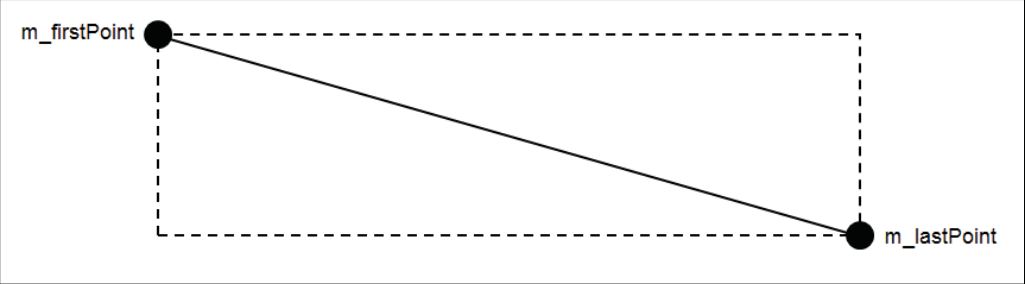
\includegraphics[width=0.85\textwidth]{images/p201_i07.png}\end{center}

\medskip\noindent{\ttfamily\bfseries Line.h}

\begin{codebox}
#ifndef LINE_H
#define LINE_H

#include <FStream>
using namespace std;

#include "Figure.h"

class Line : public Figure {
  public:
\end{codebox}

默认构造函数只在从文件读取 Line 对象时被调用；getId 只返回直线的标识枚举：

\begin{codebox}
    Line();
    FigureId getId() const {return LineId;}
\end{codebox}

直线有两个端点。两个点都在直线创建时设置，之后当用户拖动第二个点时修改它：

\begin{codebox}
    void initializePoints(QPoint point);
    void setLastPoint(QPoint point);
\end{codebox}

isClick 方法在鼠标点击位于直线上（有一定容差）时返回 true：

\begin{codebox}
    bool isClick(QPoint mousePoint);
\end{codebox}

move 方法把直线（包括两个端点）移动给定的距离：

\begin{codebox}
    void move(QSize distance);
\end{codebox}

draw 方法把直线画到 QPainter 对象上：

\begin{codebox}
    void draw(QPainter& painter) const;
\end{codebox}

write 和 read 方法从文件流写入和读取直线的端点：

\begin{codebox}
    bool write(ofstream& outStream) const;
    bool read(ifstream& inStream);
\end{codebox}

直线的首点和末点保存在 Line 对象中：

\begin{codebox}
  private:
    QPoint m_firstPoint, m_lastPoint;
  };

#endif
\end{codebox}

Line.cpp 文件定义 Line 类的方法。

\medskip\noindent{\ttfamily\bfseries Line.cpp}

\begin{codebox}
#include "..\MainWindow\DocumentWidget.h"
#include "Line.h"

Line::Line() {
  // Empty.
}
\end{codebox}

initializePoints 方法在用户向绘图添加一条新直线时被调用，它设置直线的两个端点：

\begin{codebox}
void Line::initializePoints(QPoint point) {
  m_firstPoint = point;
  m_lastPoint = point;
}
\end{codebox}

setLastPoint 方法在用户添加直线并修改其形状时被调用，它设置末点：

\begin{codebox}
void Line::setLastPoint(QPoint point) {
  m_lastPoint = point;
}
\end{codebox}

isClick 方法测试用户是否用鼠标点击了直线。有两种情形需要考虑。第一种是直线完全竖直的特殊情况，即两个端点的 x 坐标相等。我们用 Qt 的 QRect 类创建一个包围直线的矩形，并测试该点是否被矩形包围：

\begin{center}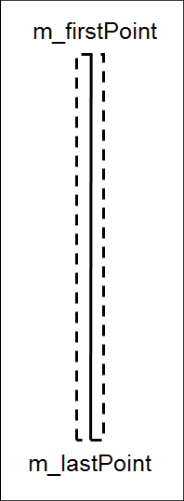
\includegraphics[width=0.3\textwidth]{images/p203_i07.png}\end{center}

\begin{codebox}
bool Line::isClick(QPoint mousePoint) {
  if (m_firstPoint.x() == m_lastPoint.x()) {
    QRect lineRect(m_firstPoint, m_lastPoint);
    lineRect.normalized();
    lineRect += Tolerance;
    return lineRect.contains(mousePoint);
  }
\end{codebox}

在直线不是竖直的一般情形中，我们首先创建一个包围矩形，并测试鼠标点是否在其中。如果在，我们把 leftPoint 设为 firstPoint 和 lastPoint 中最靠左的点，把 rightPoint 设为最靠右的点。然后计算包围矩形的宽度（lineWidth）和高度（lineHeight），以及 rightPoint 与 mousePoint 在 x 和 y 方向上的距离（diffWidth 和 diffHeight）：

\begin{center}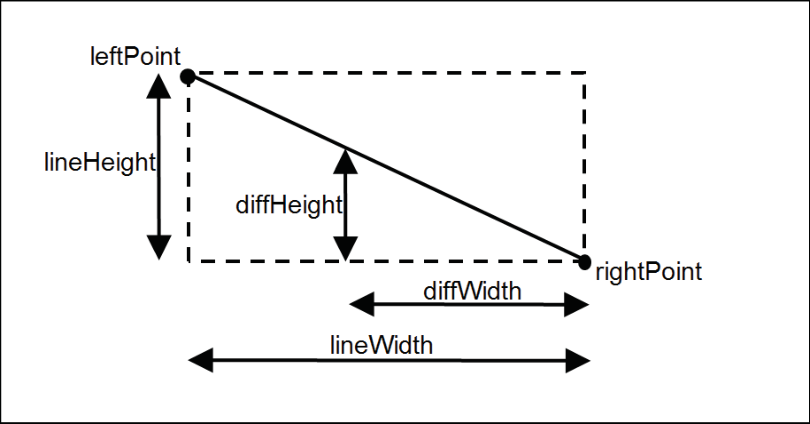
\includegraphics[width=0.85\textwidth]{images/p204_i03.png}\end{center}

根据相似性，如果鼠标指针命中直线，则下面的等式成立：

\begin{center}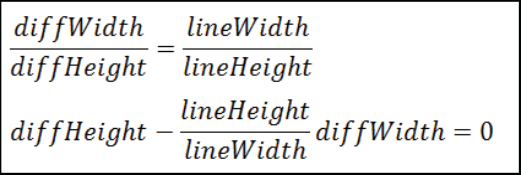
\includegraphics[width=0.5\textwidth]{images/p204_i05.png}\end{center}

不过，要让左边表达式的值恰好为零，用户必须精确地点在直线上。因此，我们允许一个小的容差，使用 Tolerance 字段：

\begin{center}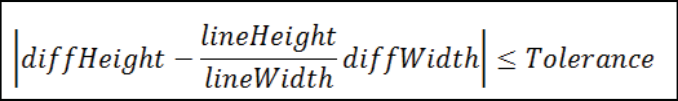
\includegraphics[width=0.6\textwidth]{images/p204_i07.png}\end{center}

\begin{codebox}
    else {
      QPoint leftPoint = (m_firstPoint.x() < m_lastPoint.x())
                         ? m_firstPoint : m_lastPoint,
             rightPoint = (m_firstPoint.x() < m_lastPoint.x())
                          ? m_lastPoint : m_firstPoint;

      if ((leftPoint.x() <= mousePoint.x()) &&
          (mousePoint.x() <= rightPoint.x())) {
        int lineWidth = rightPoint.x() - leftPoint.x(),
            lineHeight = rightPoint.y() - leftPoint.y();

        int diffWidth = mousePoint.x() - leftPoint.x(),
            diffHeight = mousePoint.y() - leftPoint.y();
\end{codebox}

我们必须把 lineHeight 转换为 double 才能进行非整数除法：

\begin{codebox}
        return (fabs(diffHeight - (((double) lineHeight) /
                     lineWidth) * diffWidth) <= Tolerance);
      }
\end{codebox}

如果鼠标点位于包围直线的矩形之外，我们直接返回 false：

\begin{codebox}
      return false;
    }
}
\end{codebox}

move 方法简单地移动直线的两个端点：

\begin{codebox}
void Line::move(QSize distance) {
  m_firstPoint += distance;
  m_lastPoint += distance;
}
\end{codebox}

绘制直线时，我们设置画笔颜色并画出直线。Figure 类的 color 方法返回直线的颜色：

\begin{codebox}
void Line::draw(QPainter& painter) const {
  painter.setPen(color());
  painter.drawLine(m_firstPoint, m_lastPoint);
}
\end{codebox}

写入直线时，我们首先调用 Figure 中的 write 来写入图形的颜色，然后写入直线的端点。最后返回输出流的布尔值——写入成功时为 true：

\begin{codebox}
bool Line::write(ofstream& outStream) const {
  Figure::write(outStream);
  writePoint(outStream, m_firstPoint);
  writePoint(outStream, m_lastPoint);
  return ((bool) outStream);
}
\end{codebox}

同样，读取直线时，我们首先调用 Figure 中的 read 来读取直线的颜色，然后读取直线的端点，并返回输入流的布尔值：

\begin{codebox}
bool Line::read(ifstream& inStream) {
  Figure::read(inStream);
  readPoint(inStream, m_firstPoint);
  readPoint(inStream, m_lastPoint);
  return ((bool) inStream);
}
\end{codebox}

\subsection{Rectangle 子类}

RectangleX 是 Figure 的子类，处理矩形。与 Line 类似，它也持有两个点，表示矩形相对的两个角：

\medskip\noindent{\ttfamily\bfseries Rectangle.h}

\begin{codebox}
#ifndef RECTANGLE_H
#define RECTANGLE_H

#include <FStream>
using namespace std;

#include "Figure.h"

class RectangleX : public Figure {
  public:
\end{codebox}

与前面的 Line 类类似，RectangleX 有一个从文件读取对象时使用的默认构造函数：

\begin{codebox}
    RectangleX();
    virtual FigureId getId() const {return RectangleId;}

    RectangleX(const RectangleX& rectangle);

    virtual void initializePoints(QPoint point);
    virtual void setLastPoint(QPoint point);
    virtual bool isClick(QPoint mousePoint);
    virtual void move(QSize distance);
    virtual void draw(QPainter& painter) const;
    virtual bool write(ofstream& outStream) const;
    virtual bool read(ifstream& inStream);
\end{codebox}

\begin{codebox}
  protected:
    QPoint m_topLeft, m_bottomRight;
  };

#endif
\end{codebox}

\medskip\noindent{\ttfamily\bfseries Rectangle.cpp}

\begin{codebox}
#include "..\MainWindow\DocumentWidget.h"
#include "Rectangle.h"

RectangleX::RectangleX() {
  // Empty.
}
\end{codebox}

initializePoints 和 setLastPoint 方法的工作方式与 Line 中的对应方法类似：initializePoints 设置两个角点，而 setLastPoint 设置最后一个角点：

\begin{codebox}
void RectangleX::initializePoints(QPoint point) {
  m_topLeft = point;
  m_bottomRight = point;
}

void RectangleX::setLastPoint(QPoint point) {
  m_bottomRight = point;
}
\end{codebox}

isClick 方法比 Line 中的对应方法简单：

\begin{codebox}
bool RectangleX::isClick(QPoint mousePoint) {
  QRect areaRect(m_topLeft, m_bottomRight);
\end{codebox}

如果矩形被填充，我们直接调用 QRect 的 contains 检查鼠标点击是否命中矩形：

\begin{codebox}
  if (filled()) {
    return areaRect.contains(mousePoint);
  }
\end{codebox}

如果矩形未被填充，我们需要检查鼠标是否点击在矩形的边框上。为此，我们创建两个稍小和稍大的矩形。如果鼠标点击命中较大的矩形而未命中较小的矩形，我们就认为点击命中了矩形边框：

\begin{codebox}
  else {
    QRect largeAreaRect(areaRect), smallAreaRect(areaRect);
    largeAreaRect += Tolerance;
    smallAreaRect -= Tolerance;
    return largeAreaRect.contains(mousePoint) &&
           !smallAreaRect.contains(mousePoint);
  }

  return false;
}
\end{codebox}

移动矩形时，我们简单地移动首末两个角点：

\begin{codebox}
void RectangleX::move(QSize distance) {
  addSizeToPoint(m_topLeft, distance);
  addSizeToPoint(m_bottomRight, distance);
}
\end{codebox}

绘制矩形时，我们首先通过调用 Figure 中的 color 设置画笔颜色：

\begin{codebox}
void RectangleX::draw(QPainter& painter) const {
  painter.setPen(color());
\end{codebox}

如果矩形被填充，我们直接调用 QPainter 对象的 fillRect：

\begin{codebox}
  if (filled()) {
    painter.fillRect(QRect(m_topLeft, m_bottomRight), color());
  }
\end{codebox}

如果矩形未被填充，我们禁用画刷使矩形成为空心，然后调用 QPainter 对象的 drawRect 画出矩形边框：

\begin{codebox}
  else {
    painter.setBrush(Qt::NoBrush);
    painter.drawRect(QRect(m_topLeft, m_bottomRight));
  }
}
\end{codebox}

write 方法首先调用 Figure 中的 write，然后写入矩形的首末角点：

\begin{codebox}
bool RectangleX::write(ofstream& outStream) const {
  Figure::write(outStream);
  writePoint(outStream, m_topLeft);
  writePoint(outStream, m_bottomRight);
  return ((bool) outStream);
}
\end{codebox}

同样，read 首先调用 Figure 中的 read，然后读取矩形的首末角点：

\begin{codebox}
bool RectangleX::read (ifstream& inStream) {
  Figure::read(inStream);
  readPoint(inStream, m_topLeft);
  readPoint(inStream, m_bottomRight);
  return ((bool) inStream);
}
\end{codebox}

\subsection{Ellipse 子类}

EllipseX 是 RectangleX 的子类，处理椭圆。RectangleX 的部分功能在 EllipseX 中得到复用。更具体地说，initializePoints、setLastPoint、move、write 和 read 都是从 RectangleX 重写而来的。

\medskip\noindent{\ttfamily\bfseries Ellipse.h}

\begin{codebox}
#ifndef ELLIPSE_H
#define ELLIPSE_H

#include "Rectangle.h"

class EllipseX : public RectangleX {
  public:
    EllipseX();
    FigureId getId() const {return EllipseId;}

    EllipseX(const EllipseX& ellipse);

    bool isClick(QPoint mousePoint);
    void draw(QPainter& painter) const;
  };

#endif
\end{codebox}

\medskip\noindent{\ttfamily\bfseries Ellipse.cpp}

\begin{codebox}
#include "..\MainWindow\DocumentWidget.h"
#include "Ellipse.h"

EllipseX::EllipseX() {
  // Empty.
}
\end{codebox}

EllipseX 的 isClick 方法与 RectangleX 中的对应方法类似。我们用 Qt 的 QRegion 类创建椭圆区域，并把它们与鼠标点击进行比较：

\begin{codebox}
bool EllipseX::isClick(QPoint mousePoint) {
  QRect normalRect(m_topLeft, m_bottomRight);
  normalRect.normalized();
\end{codebox}

如果椭圆被填充，我们创建一个椭圆区域并测试鼠标点击是否命中该区域：

\begin{codebox}
  if (filled()) {
    QRegion normalEllipse(normalRect, QRegion::Ellipse);
    return normalEllipse.contains(mousePoint);
  }
\end{codebox}

如果椭圆未被填充，我们创建稍小和稍大的椭圆区域。如果鼠标点击命中较大的区域而未命中较小的区域，我们就认为点击命中了椭圆边框：

\begin{codebox}
  else {
    QRect largeRect(normalRect), smallRect(normalRect);
    largeRect += Tolerance;
    smallRect -= Tolerance;

    QRegion largeEllipse(largeRect, QRegion::Ellipse),
            smallEllipse(smallRect, QRegion::Ellipse);

    return (largeEllipse.contains(mousePoint) &&
            !smallEllipse.contains(mousePoint));
  }
}
\end{codebox}

绘制椭圆时，我们首先通过调用 Figure 中的 color 设置画笔颜色：

\begin{codebox}
void EllipseX::draw(QPainter& painter) const {
  painter.setPen(color());
\end{codebox}

如果椭圆被填充，我们设置画刷并绘制椭圆：

\begin{codebox}
  if (filled()) {
    painter.setBrush(color());
    painter.drawEllipse(QRect(m_topLeft, m_bottomRight));
  }
\end{codebox}

如果椭圆未被填充，我们把画刷设为空心并绘制椭圆边框：

\begin{codebox}
  else {
    painter.setBrush(Qt::NoBrush);
    painter.drawEllipse(QRect(m_topLeft, m_bottomRight));
  }
}
\end{codebox}

\subsection{绘制窗口}

DrawingWindow 类是上一节 MainWindow 类的子类。

\medskip\noindent{\ttfamily\bfseries DrawingWindow.h}

\begin{codebox}
#ifndef DRAWINGWINDOW_H
#define DRAWINGWINDOW_H

#include <QMainWindow>
#include <QActionGroup>

#include "..\MainWindow\MainWindow.h"
#include "DrawingWidget.h"

class DrawingWindow : public MainWindow {
  Q_OBJECT

  public:
    DrawingWindow(QWidget* parentWidgetPtr = nullptr);
    ~DrawingWindow();

  public:
    void closeEvent(QCloseEvent *eventPtr)
         { m_drawingWidgetPtr->closeEvent(eventPtr); }

  private:
    DrawingWidget* m_drawingWidgetPtr;
    QActionGroup* m_figureGroupPtr;
  };

#endif // DRAWINGWINDOW_H
\end{codebox}

\medskip\noindent{\ttfamily\bfseries DrawingWindow.cpp}

\begin{codebox}
#include "..\MainWindow\DocumentWidget.h"
#include "DrawingWindow.h"
\end{codebox}

构造函数把窗口大小设为 1000 $\times$ 500 像素：

\begin{codebox}
DrawingWindow::DrawingWindow(QWidget* parentWidgetPtr
                             /* = nullptr */)
 :MainWindow(parentWidgetPtr) {
  resize(1000, 500);
\end{codebox}

m\_drawingWidgetPtr 字段初始化为指向一个 DrawingWidget 类的对象，该对象随后被设置为窗口的中央部分：

\begin{codebox}
  m_drawingWidgetPtr = new DrawingWidget(this);
  setCentralWidget(m_drawingWidgetPtr);
\end{codebox}

标准 File 菜单被添加到窗口菜单栏：

\begin{codebox}
  addFileMenu();
\end{codebox}

然后我们添加应用专属的 Format 菜单。它与上一节 DocumentWidget 类的 onMenuShow 方法连接：

\begin{codebox}
  { QMenu* formatMenuPtr = menuBar()->addMenu(tr("F&ormat"));
    connect(formatMenuPtr, SIGNAL(aboutToShow()),
            this, SLOT(onMenuShow()));
\end{codebox}

Format 菜单包含颜色和填充菜单项：

\begin{codebox}
    addAction(formatMenuPtr, tr("&Color"),
              SLOT(onColor()), QKeySequence(Qt::ALT + Qt::Key_C),
              QString(), nullptr, tr("Figure Color"));
\end{codebox}

当画图程序的下一个图形是二维图形（矩形或椭圆）时，Fill 菜单项才会启用：

\begin{codebox}
    addAction(formatMenuPtr, tr("&Fill"),
              SLOT(onFill()), QKeySequence(Qt::CTRL + Qt::Key_F),
              QString(), nullptr, tr("Figure Fill"),
              LISTENER(isFillEnabled));
  }
\end{codebox}

对于图形菜单，我们为直线、矩形和椭圆菜单项创建一个新的动作组。同一时刻它们之中只能有一个被选中：

\begin{codebox}
  { m_figureGroupPtr = new QActionGroup(this);

    QMenu* figureMenuPtr = menuBar()->addMenu(tr("F&igure"));
    connect(figureMenuPtr, SIGNAL(aboutToShow()),
            this, SLOT(onMenuShow()));
\end{codebox}

当前选中的菜单项应标注单选按钮：

\begin{codebox}
    addAction(figureMenuPtr, tr("&Line"),
              SLOT(onLine()), QKeySequence(Qt::CTRL + Qt::Key_L),
              QString(), nullptr, tr("Line Figure"), nullptr,
              LISTENER(isLineChecked), m_figureGroupPtr);
    addAction(figureMenuPtr, tr("&Rectangle"),
              SLOT(onRectangle()),
              QKeySequence(Qt::CTRL + Qt::Key_R),
              QString(), nullptr, tr("Rectangle Figure"), nullptr,
              LISTENER(isRectangleChecked), m_figureGroupPtr);
    addAction(figureMenuPtr, tr("&Ellipse"),
              SLOT(onEllipse()),
              QKeySequence(Qt::CTRL + Qt::Key_E),
              QString(), nullptr, tr("Ellipse Figure"), nullptr,
              LISTENER(isEllipseChecked), m_figureGroupPtr);
  }
}
\end{codebox}

析构函数释放构造函数中动态分配的图形组：

\begin{codebox}
DrawingWindow::~DrawingWindow() {
  delete m_figureGroupPtr;
}
\end{codebox}

\subsection{绘制部件}

DrawingWidget 是上一节 DocumentWidget 的子类。它处理鼠标输入、图形的绘制以及绘图的保存和加载，还提供决定菜单项何时应被标记和启用的方法。

\medskip\noindent{\ttfamily\bfseries DrawingWidget.h}

\begin{codebox}
#ifndef DRAWINGWIDGET_H
#define DRAWINGWIDGET_H

#include "..\MainWindow\MainWindow.h"
#include "..\MainWindow\DocumentWidget.h"
#include "Figure.h"

class DrawingWidget : public DocumentWidget {
  Q_OBJECT

  public:
    DrawingWidget(QWidget* parentWidgetPtr);
    ~DrawingWidget();
\end{codebox}

mousePressEvent、mouseReleaseEvent 和 mouseMoveEvent 是重写的方法，在用户按下或松开某个鼠标键或移动鼠标时被调用：

\begin{codebox}
  public:
    void mousePressEvent(QMouseEvent *eventPtr);
    void mouseReleaseEvent(QMouseEvent *eventPtr);
    void mouseMoveEvent(QMouseEvent *eventPtr);
\end{codebox}

paintEvent 方法在窗口需要重绘时被调用。原因可能有多种，例如用户可以改变窗口大小。重绘也可以由对 update 方法的调用强制触发，该调用最终会导致 paintEvent 被调用：

\begin{codebox}
    void paintEvent(QPaintEvent *eventPtr);
\end{codebox}

用户选择 New 菜单项时调用 newDocument 方法，选择 save 或 save as 菜单项时调用 writeFile，选择 open 菜单项时调用 readFile：

\begin{codebox}
  private:
    void newDocument() override;
    bool writeFile(const QString& filePath);
    bool readFile(const QString& filePath);
    Figure* createFigure(FigureId figureId);
\end{codebox}

用户选择颜色和填充菜单项时调用 onColor 和 onFill 方法：

\begin{codebox}
  public slots:
    void onColor();
    void onFill();
\end{codebox}

isFillEnabled 方法在用户选择 Format 菜单之前被调用。如果它返回 true，Fill 菜单项就会被启用：

\begin{codebox}
    DEFINE_LISTENER(DrawingWidget, isFillEnabled);
\end{codebox}

isLineChecked、isRectangleChecked 和 isEllipseChecked 方法也在 Figure 菜单可见之前被调用。如果这些方法返回 true，相应的菜单项就会标注单选按钮：

\begin{codebox}
    DEFINE_LISTENER(DrawingWidget, isLineChecked);
    DEFINE_LISTENER(DrawingWidget, isRectangleChecked);
    DEFINE_LISTENER(DrawingWidget, isEllipseChecked);
\end{codebox}

用户选择直线、矩形和椭圆菜单项时调用 onLine、onRectangle 和 onEllipse 方法：

\begin{codebox}
    void onLine();
    void onRectangle();
    void onEllipse();
\end{codebox}

运行时，应用可以处于 Idle、Create 或 Move 三种模式：

\begin{itemize}
\item \textbf{Idle}：应用等待用户输入。
\item \textbf{Create}：用户正在向绘图添加新图形。发生在用户按下鼠标左键且未命中任何图形时。此时会添加一个新图形，并修改其端点，直到用户松开鼠标键。
\item \textbf{Move}：用户正在移动一个图形。发生在用户按下鼠标左键并命中某个图形时。该图形被移动，直到用户松开鼠标键。
\end{itemize}

\begin{codebox}
  private:
    enum ApplicationMode {Idle, Create, Move};
    ApplicationMode m_applicationMode = Idle;
    void setApplicationMode(ApplicationMode mode);
\end{codebox}

m\_currColor 字段保存用户接下来要添加的图形的颜色；m\_currFilled 决定下一个图形（如果是矩形或椭圆）是否被填充。m\_addFigureId 字段保存用户接下来要添加的图形类型（直线、矩形或椭圆）的标识整数：

\begin{codebox}
    QColor m_currColor = Qt::black;
    bool m_currFilled = false;
    FigureId m_addFigureId = LineId;
\end{codebox}

用户按下鼠标键并移动图形时，我们需要保存之前的鼠标点，以便计算自上次鼠标事件以来图形移动的距离：

\begin{codebox}
    QPoint m_mousePoint;
\end{codebox}

最后，m\_figurePtrList 保存指向绘图中各图形的指针。绘图中最上层的图形位于列表末尾：

\begin{codebox}
    QList<Figure*> m_figurePtrList;
  };

#endif // DRAWINGWIDGET_H
\end{codebox}

\medskip\noindent{\ttfamily\bfseries DrawingWidget.cpp}

\begin{codebox}
#include "..\MainWindow\DocumentWidget.h"
#include "DrawingWidget.h"

#include "Line.h"
#include "Rectangle.h"
#include "Ellipse.h"
\end{codebox}

构造函数调用基类 DocumentWidget 的构造函数，标题为 Drawing；它还把保存和加载掩码设为 Drawing files (*.drw)，也就是说标准保存和加载对话框默认选择的文件以后缀 drw 结尾：

\begin{codebox}
DrawingWidget::DrawingWidget(QWidget* parentWidgetPtr)
 :DocumentWidget(tr("Drawing"), tr("Drawing files (*.drw)"),
                 parentWidgetPtr) {
  // Empty.
}
\end{codebox}

析构函数释放图形指针列表中的图形指针：

\begin{codebox}
DrawingWidget::~DrawingWidget() {
  for (Figure* figurePtr : m_figurePtrList) {
    delete figurePtr;
  }
}
\end{codebox}

setApplicationMode 方法设置应用模式，并调用主窗口的 onMenuShow，使工具栏图标被正确启用：

\begin{codebox}
void DrawingWidget::setApplicationMode(ApplicationMode mode) {
  m_applicationMode = mode;
  ((MainWindow*) parent())->onMenuShow();
}
\end{codebox}

用户选择 New 菜单项时调用 newDocument。图形指针列表中的图形被释放，列表本身也被清空。用户接下来要添加的图形是一条黑色直线，填充状态为 false：

\begin{codebox}
void DrawingWidget::newDocument() {
  for (Figure* figurePtr : m_figurePtrList) {
    delete figurePtr;
  }
  m_figurePtrList.clear();

  m_currColor = Qt::black;
  m_addFigureId = LineId;
  m_currFilled = false;
}
\end{codebox}

用户选择 save 或 save as 菜单项时调用 writeFile 方法：

\begin{codebox}
bool DrawingWidget::writeFile(const QString& filePath) {
  ofstream outStream(filePath.toStdString());
\end{codebox}

我们首先写入当前的颜色和填充状态，然后写入图形指针列表的大小以及各图形本身：

\begin{codebox}
  if (outStream) {
    writeColor(outStream, m_currColor);
    outStream.write((char*) &m_currFilled, sizeof m_currFilled);

    int size = m_figurePtrList.size();
    outStream.write((char*) &size, sizeof size);
\end{codebox}

对每个图形，我们先写入它的标识号，再写入图形本身：

\begin{codebox}
    for (Figure* figurePtr : m_figurePtrList) {
      FigureId figureId = figurePtr->getId();
      outStream.write((char*) &figureId, sizeof figureId);
      figurePtr->write(outStream);
    }

    return ((bool) outStream);
  }
\end{codebox}

如果文件无法打开，则返回 false：

\begin{codebox}
  return false;
}
\end{codebox}

用户选择 open 菜单项时调用 readFile 方法。与前面的 writeFile 一样，我们读取颜色和填充状态、图形指针列表的大小以及各图形本身：

\begin{codebox}
bool DrawingWidget::readFile(const QString& filePath) {
  ifstream inStream(filePath.toStdString());

  if (inStream) {
    readColor(inStream, m_currColor);
    inStream.read((char*) &m_currFilled, sizeof m_currFilled);

    int size;
    inStream.read((char*) &size, sizeof size);
\end{codebox}

读取图形时，我们先读取它的标识号，然后调用 createFigure 创建一个与该图形标识号对应的类的对象。接着调用图形指针上的 read 读取图形的字段。注意，我们其实并不知道（也不关心）它是哪种图形。我们只是简单地调用图形指针的 read，而这个指针实际上指向 Line、RectangleX 或 EllipseX 的对象：

\begin{codebox}
    for (int count = 0; count < size; ++count) {
      FigureId figureId = (FigureId) 0;
      inStream.read((char*) &figureId, sizeof figureId);
      Figure* figurePtr = createFigure(figureId);
      figurePtr->read(inStream);
      m_figurePtrList.push_back(figurePtr);
    }

    return ((bool) inStream);
  }

  return false;
}
\end{codebox}

createFigure 方法根据 figureId 参数的值动态创建 Line、RectangleX 或 EllipseX 类的对象：

\begin{codebox}
Figure* DrawingWidget::createFigure(FigureId figureId) {
  Figure* figurePtr = nullptr;

  switch (figureId) {
    case LineId:
      figurePtr = new Line();
      break;

    case RectangleId:
      figurePtr = new RectangleX();
      break;

    case EllipseId:
      figurePtr = new EllipseX();
      break;
  }

  return figurePtr;
}
\end{codebox}

用户选择颜色菜单项时调用 onColor 方法。它设置用户接下来要添加的图形的颜色：

\begin{codebox}
void DrawingWidget::onColor() {
  QColor newColor = QColorDialog::getColor(m_currColor, this);

  if (newColor.isValid() && (m_currColor != newColor)) {
    m_currColor = newColor;
    setModifiedFlag(true);
  }
}
\end{codebox}

isFillEnabled 方法在 Format 菜单可见之前被调用，如果用户接下来要添加的图形是矩形或椭圆，它返回 true：

\begin{codebox}
bool DrawingWidget::isFillEnabled() {
  return (m_addFigureId == RectangleId) ||
         (m_addFigureId == EllipseId);
}
\end{codebox}

用户选择填充菜单项时调用 onFill 方法。它把 m\_currFilled 字段取反。由于文档已受影响，它还设置 modified 标志：

\begin{codebox}
void DrawingWidget::onFill() {
  m_currFilled = !m_currFilled;
  setModifiedFlag(true);
}
\end{codebox}

isLineChecked、isRectangleChecked 和 isEllipseChecked 方法在 Figure 菜单可见之前被调用。如果用户接下来要添加的图形正是相应图形，它们返回 true，菜单项就会标注单选按钮：

\begin{codebox}
bool DrawingWidget::isLineChecked() {
  return (m_addFigureId == LineId);
}

bool DrawingWidget::isRectangleChecked() {
  return (m_addFigureId == RectangleId);
}

bool DrawingWidget::isEllipseChecked() {
  return (m_addFigureId == EllipseId);
}
\end{codebox}

用户选择 Figure 菜单中的菜单项时调用 onLine、onRectangle 和 onEllipse 方法。它们把用户接下来要添加的图形设置为相应的图形：

\begin{codebox}
void DrawingWidget::onLine() {
  m_addFigureId = LineId;
}

void DrawingWidget::onRectangle() {
  m_addFigureId = RectangleId;
}

void DrawingWidget::onEllipse() {
  m_addFigureId = EllipseId;
}
\end{codebox}

用户每次按下某个鼠标键时都会调用 mousePressEvent 方法。首先，我们需要检查用户按下的是否是鼠标左键：

\begin{codebox}
void DrawingWidget::mousePressEvent(QMouseEvent* eventPtr) {
  if (eventPtr->buttons() == Qt::LeftButton) {
\end{codebox}

在下面代码片段中对 mouseMoveEvent 的调用中，我们需要记录最新的鼠标点，以便计算鼠标移动之间的距离。因此，我们把 m\_mousePoint 设为该鼠标点：

\begin{codebox}
    m_mousePoint = eventPtr->pos();
\end{codebox}

我们遍历图形指针列表，对每个图形调用 isClick，检查该图形是否被鼠标点击命中。我们需要以一种比较别扭的方式反向遍历，以便先找到最上层的图形。我们使用 reverse\_iterator 类以及 rbegin 和 rend 方法来反向遍历：

\begin{codebox}
    for (QList<Figure*>::reverse_iterator iterator =
         m_figurePtrList.rbegin();
         iterator != m_figurePtrList.rend(); ++iterator) {
\end{codebox}

我们用解引用运算符（\texttt{*}）取得列表中的图形指针：

\begin{codebox}
        Figure* figurePtr = *iterator;
\end{codebox}

如果该图形被鼠标点击命中，我们把应用模式设为 Move，并通过调用列表的 removeOne 和 push\_back 把该图形移到列表末尾，使它在绘图中显示为最上层。最后，我们中断循环，因为已经找到了要找的图形：

\begin{codebox}
        if (figurePtr->isClick(m_mousePoint)) {
          setApplicationMode(Move);
          m_figurePtrList.removeOne(figurePtr);
          m_figurePtrList.push_back(figurePtr);
          break;
        }
      }
\end{codebox}

如果应用模式仍是 Idle（未发生移动），说明没有图形被鼠标点击命中。此时我们把应用模式设为 Create，并调用 createFigure 找一个图形来复制。然后设置该图形的颜色、填充状态以及各点。最后，我们调用 push\_back 把图形指针加入图形指针列表（它被加到列表末尾，以便显示在绘图最上层），并把 modified 标志设为 true，因为绘图已被修改：

\begin{codebox}
      if (m_applicationMode == Idle) {
        setApplicationMode(Create);
        Figure* newFigurePtr = createFigure(m_addFigureId);
        newFigurePtr->color() = m_currColor;
        newFigurePtr->filled() = m_currFilled;
        newFigurePtr->initializePoints(m_mousePoint);
        m_figurePtrList.push_back(newFigurePtr);
        setModifiedFlag(true);
      }
    }
}
\end{codebox}

用户每次移动鼠标时都会调用 mouseMoveEvent。首先，我们需要检查用户移动鼠标时按下的是否是鼠标左键：

\begin{codebox}
void DrawingWidget::mouseMoveEvent(QMouseEvent* eventPtr) {
  if (eventPtr->buttons() == Qt::LeftButton) {
    QPoint newMousePoint = eventPtr->pos();
\end{codebox}

然后检查应用模式。如果我们正在向绘图添加新图形，就修改它的末点：

\begin{codebox}
    switch (m_applicationMode) {
      case Create:
        m_figurePtrList.back()->setLastPoint(m_mousePoint);
        break;
\end{codebox}

如果我们正在移动一个图形，我们计算自上次鼠标事件以来的距离，并移动位于图形指针列表末尾的图形。记住，在前面 mousePressEvent 中被鼠标点击命中的图形已被移到图形指针列表的末尾：

\begin{codebox}
      case Move: {
          QSize distance(newMousePoint.x() - m_mousePoint.x(),
                         newMousePoint.y() - m_mousePoint.y());
          m_figurePtrList.back()->move(distance);
          setModifiedFlag(true);
        }
        break;
    }
\end{codebox}

最后，我们更新当前鼠标点，供下一次调用 mouseMoveEvent 使用。我们还调用 update 方法强制重绘窗口：

\begin{codebox}
    m_mousePoint = newMousePoint;
    update();
  }
}
\end{codebox}

用户松开某个鼠标键时调用 mouseReleaseEvent 方法。我们把应用模式设为 Idle：

\begin{codebox}
void DrawingWidget::mouseReleaseEvent(QMouseEvent* eventPtr) {
  if (eventPtr->buttons() == Qt::LeftButton) {
    setApplicationMode(Idle);
  }
}
\end{codebox}

每当窗口需要重绘时就会调用 paintEvent 方法。原因可能有多种：例如用户可能改变了窗口大小；也可能是 Qt QWidget 类中 update 调用的结果——它强制重绘窗口，并最终调用 paintEvent。

我们首先创建一个 QPainter 对象——它可以看作一块画布——并设置合适的渲染方式。然后遍历图形指针列表，绘制每个图形。这样，列表中的最后一个图形绘制在绘图的最上层：

\begin{codebox}
void DrawingWidget::paintEvent(QPaintEvent* /* eventPtr */) {
  QPainter painter(this);
  painter.setRenderHint(QPainter::Antialiasing);
  painter.setRenderHint(QPainter::TextAntialiasing);

  for (Figure* figurePtr : m_figurePtrList) {
    figurePtr->draw(painter);
  }
}
\end{codebox}

\subsection{main 函数}

最后，我们在 main 函数中启动应用程序：创建应用对象，显示主窗口，并执行应用。

\medskip\noindent{\ttfamily\bfseries Main.cpp}

\begin{codebox}
#include "DrawingWindow.h"
#include <QApplication>

int main(int argc, char *argv[]) {
  QApplication application(argc, argv);
  DrawingWindow drawingWindow;
  drawingWindow.show();
  return application.exec();
}
\end{codebox}

得到如下输出：

\begin{center}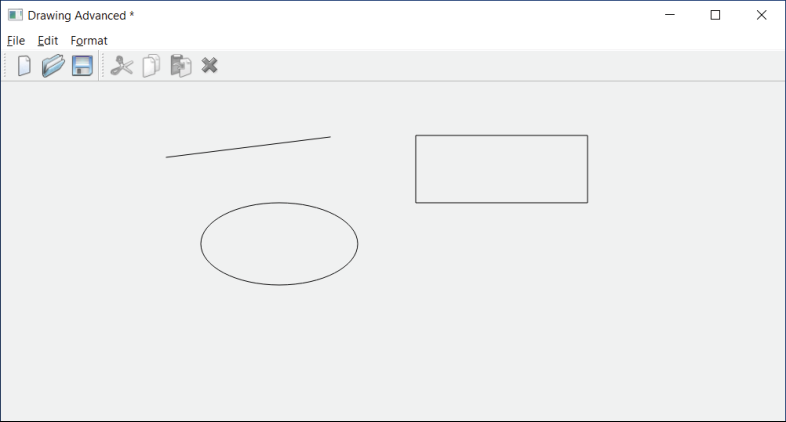
\includegraphics[width=0.9\textwidth]{images/p224_i03.png}\end{center}

\section{构建编辑器}

下一个应用是编辑器，用户可以在其中输入和编辑文本。当前的输入位置由插入符（caret）指示。可以用方向键移动插入符，也可以用鼠标点击移动。

\subsection{Caret 类}

Caret 类处理插入符，也就是标记下一个输入字符位置的闪烁竖线。

\medskip\noindent{\ttfamily\bfseries Caret.h}

\begin{codebox}
#ifndef CARET_H
#define CARET_H

#include <QObject>
#include <QWidget>
#include <QTimer>

class Caret : public QObject {
  Q_OBJECT

  public:
    Caret(QWidget* parentWidgetPtr = nullptr);
\end{codebox}

show 和 hide 方法显示和隐藏插入符。本应用中插入符从不隐藏；不过下一章的高级版本中，插入符在某些情况下会被隐藏：

\begin{codebox}
    void show();
    void hide();
\end{codebox}

set 方法设置插入符的当前大小和位置，paint 则把插入符画到 QPainter 对象上：

\begin{codebox}
    void set(QRect rect);
    void paint(QPainter& painter);
\end{codebox}

插入符每次闪烁时都会调用 onTimer 方法：

\begin{codebox}
  public slots:
    void onTimer(void);

  private:
    QWidget* m_parentWidgetPtr;
\end{codebox}

插入符可见时 m\_visible 字段为 true：

\begin{codebox}
    bool m_visible, m_blink;
\end{codebox}

m\_rect 字段保存插入符的矩形区域；让插入符闪烁的定时器由 m\_timer 字段处理：

\begin{codebox}
    QRect m_rect;
    QTimer m_timer;
  };

#endif // CARET_H
\end{codebox}

Caret.cpp 文件存放 Caret 类方法的定义。

\medskip\noindent{\ttfamily\bfseries Caret.cpp}

\begin{codebox}
#include "Caret.h"
#include <QPainter>
\end{codebox}

构造函数把定时器信号连接到 onTimer，其效果是每次超时都会调用 onTimer。定时器随后被初始化为 500 毫秒。也就是说，onTimer 每 500 毫秒被调用一次，插入符每 500 毫秒显示和隐藏一次：

\begin{codebox}
Caret::Caret(QWidget* parentWidgetPtr)
  :m_parentWidgetPtr(parentWidgetPtr) {
  m_timer.setParent(this);
  connect(&m_timer, SIGNAL(timeout()), this, SLOT(onTimer()));
  m_timer.start(500);
}
\end{codebox}

show 和 hide 方法设置 m\_visible 字段，并通过在父窗口上调用 update 强制重绘插入符区域：

\begin{codebox}
void Caret::show() {
  m_visible = true;
  m_parentWidgetPtr->update(m_rect);
}

void Caret::hide() {
  m_visible = false;
  m_parentWidgetPtr->update(m_rect);
}
\end{codebox}

set 方法设置插入符的大小和位置。不过，插入符的宽度总是设为 1，这使它看起来像一条细竖线：

\begin{codebox}
void Caret::set(QRect rect) {
  m_rect = rect;
  m_rect.setWidth(1);
  m_parentWidgetPtr->update(m_rect);
}
\end{codebox}

onTimer 方法每 500 毫秒被调用一次。它把 m\_blink 取反并强制重绘插入符。结果是插入符以一秒的间隔闪烁：

\begin{codebox}
void Caret::onTimer(void) {
  m_blink = !m_blink;
  m_parentWidgetPtr->update(m_rect);
}
\end{codebox}

每当插入符需要重绘时就会调用 paint 方法。只有 m\_visible 和 m\_blink 都为 true 时才绘制插入符——即插入符被设为可见且正处于闪烁的可见区间。调用 paint 之前插入符区域会被清空，因此如果没有绘制发生，插入符就被清除：

\begin{codebox}
void Caret::paint(QPainter& painter) {
  if (m_visible && m_blink) {
    painter.save();
    painter.setPen(Qt::NoPen);
    painter.setBrush(Qt::black);
    painter.drawRect(m_rect);
    painter.restore();
  }
}
\end{codebox}

\subsection{绘制编辑器窗口}

EditorWindow 是上一节 MainWindow 类的子类。它处理窗口的关闭，还处理按键事件。

\medskip\noindent{\ttfamily\bfseries EditorWindow.h}

\begin{codebox}
#ifndef EDITORWINDOW_H
#define EDITORWINDOW_H

#include <QMainWindow>
#include <QActionGroup>
#include <QPair>
#include <QMap>

#include "..\MainWindow\MainWindow.h"
#include "EditorWidget.h"

class EditorWindow : public MainWindow {
  Q_OBJECT

  public:
    EditorWindow(QWidget* parentWidgetPtr = nullptr);
    ~EditorWindow();
\end{codebox}

用户每次按下按键都会调用 keyPressEvent 方法；用户试图关闭窗口时调用 closeEvent 方法：

\begin{codebox}
  protected:
    void keyPressEvent(QKeyEvent* eventPtr);
    void closeEvent(QCloseEvent* eventPtr);

  private:
    EditorWidget* m_editorWidgetPtr;
  };

#endif // EDITORWINDOW_H
\end{codebox}

EditorWindow 类实际上相当小。它只定义了构造函数和析构函数，以及 keyPressEvent 和 closeEvent 方法。

\medskip\noindent{\ttfamily\bfseries EditorWindow.cpp}

\begin{codebox}
#include "EditorWindow.h"
#include <QtWidgets>
\end{codebox}

构造函数把窗口大小设为 1000 $\times$ 500 像素，并把标准 File 菜单添加到菜单栏：

\begin{codebox}
EditorWindow::EditorWindow(QWidget* parentWidgetPtr /*= nullptr*/)
 :MainWindow(parentWidgetPtr) {
  resize(1000, 500);
  m_editorWidgetPtr = new EditorWidget(this);
  setCentralWidget(m_editorWidgetPtr);
  addFileMenu();
}

EditorWindow::~EditorWindow() {
  // Empty.
}
\end{codebox}

keyPressEvent 和 closeEvent 方法只是把消息转发给位于窗口中央的编辑器部件中的对应方法：

\begin{codebox}
void EditorWindow::keyPressEvent(QKeyEvent* eventPtr) {
  m_editorWidgetPtr->keyPressEvent(eventPtr);
}

void EditorWindow::closeEvent(QCloseEvent* eventPtr) {
  m_editorWidgetPtr->closeEvent(eventPtr);
}
\end{codebox}

\subsection{绘制编辑器部件}

EditorWidget 类是上一节 DocumentWidget 的子类。它捕获按键、鼠标、窗口大小改变和关闭事件，还重写了保存和加载文档的方法。

\medskip\noindent{\ttfamily\bfseries EditorWidget.h}

\begin{codebox}
#ifndef EDITORWIDGET_H
#define EDITORWIDGET_H

#include <QWidget>
#include <QMap>
#include <QMenu>
#include <QToolBar>
#include <QPair>

#include "Caret.h"
#include "..\MainWindow\DocumentWidget.h"

class EditorWidget : public DocumentWidget {
  Q_OBJECT

  public:
    EditorWidget(QWidget* parentWidgetPtr);
\end{codebox}

用户按下按键时调用 keyPressEvent，用户点击鼠标时调用 mousePressEvent：

\begin{codebox}
    void keyPressEvent(QKeyEvent* eventPtr);
    void mousePressEvent(QMouseEvent* eventPtr);
\end{codebox}

mouseToIndex 是一个辅助方法，计算用户用鼠标点击的字符的索引：

\begin{codebox}
  private:
    int mouseToIndex(QPoint point);
\end{codebox}

窗口需要重绘时调用 paintEvent 方法，用户改变窗口大小时调用 resizeEvent 方法。本应用中我们捕获窗口大小改变事件，是因为要重新计算每行能容纳的字符数：

\begin{codebox}
  public:
    void paintEvent(QPaintEvent* eventPtr);
    void resizeEvent(QResizeEvent* eventPtr);
\end{codebox}

与上一节的画图程序类似，用户选择 New 菜单项时调用 newDocument，选择 save 或 save as 菜单项时调用 writeFile，选择 open 菜单项时调用 readFile：

\begin{codebox}
  private:
    void newDocument(void);
    bool writeFile(const QString& filePath);
    bool readFile(const QString& filePath);
\end{codebox}

响应用户输入或鼠标点击而设置插入符时调用 setCaret 方法：

\begin{codebox}
  private:
    void setCaret();
\end{codebox}

用户上移或下移插入符时，我们需要找到插入符上方或下方字符的索引。最简单的办法是模拟一次鼠标点击：

\begin{codebox}
    void simulateMouseClick(int x, int y);
\end{codebox}

calculate 是一个辅助方法，计算行数以及每行中每个字符的位置：

\begin{codebox}
  private:
    void calculate();
\end{codebox}

m\_editIndex 字段保存用户输入文本的位置的索引。该位置也是插入符可见的位置：

\begin{codebox}
    int m_editIndex = 0;
\end{codebox}

m\_caret 字段保存应用的插入符：

\begin{codebox}
    Caret m_caret;
\end{codebox}

编辑器的文本保存在 m\_editorText 中：

\begin{codebox}
    QString m_editorText;
\end{codebox}

编辑器的文本可能分布在多行上；m\_lineList 记录每一行的首末索引：

\begin{codebox}
    QList<QPair<int,int>> m_lineList;
\end{codebox}

前面提到的 calculate 方法计算编辑器文本中每个字符的矩形，并把它们放入 m\_rectList：

\begin{codebox}
    QList<QRect> m_rectList;
\end{codebox}

本章的应用中所有字符使用同一字体，保存在 TextFont 中：

\begin{codebox}
    static const QFont TextFont;
\end{codebox}

FontWidth 和 FontHeight 保存 TextFont 中一个字符的宽度和高度：

\begin{codebox}
    int FontWidth, FontHeight;
  };

#endif // EDITORWIDGET_H
\end{codebox}

EditorWidget 类相当庞大，它定义编辑器的功能。

\medskip\noindent{\ttfamily\bfseries EditorWidget.cpp}

\begin{codebox}
#include "EditorWidget.h"
#include <QtWidgets>
using namespace std;
\end{codebox}

我们把文本字体初始化为 12 磅的 Courier New：

\begin{codebox}
const QFont EditorWidget::TextFont("Courier New", 12);
\end{codebox}

构造函数把标题设为 Editor，并把标准 Load 和 Save 对话框的文件后缀设为 edi。文本字体中一个字符的高度和平均宽度（像素）用 Qt 的 QFontMetrics 类取得。计算每个字符的矩形，并把插入符设到文本的第一个字符上：

\begin{codebox}
EditorWidget::EditorWidget(QWidget* parentWidgetPtr)
 :DocumentWidget(tr("Editor"), tr("Editor files (*.edi)"),
                 parentWidgetPtr),
  m_caret(this),
  m_editorText(tr("Hello World")) {
  QFontMetrics metrics(TextFont);
  FontHeight = metrics.height();
  FontWidth = metrics.averageCharWidth();
  calculate();
  setCaret();
  m_caret.show();
}
\end{codebox}

用户选择 New 菜单项时调用 newDocument 方法。它清空文本、设置插入符并重新计算字符矩形：

\begin{codebox}
void EditorWidget::newDocument(void) {
  m_editIndex = 0;
  m_editorText.clear();
  calculate();
  setCaret();
}
\end{codebox}

用户选择 save 或 save as 菜单项时调用 writeFile 方法。它简单地写出编辑器当前文本：

\begin{codebox}
bool EditorWidget::writeFile(const QString& filePath) {
  QFile file(filePath);
  if (file.open(QIODevice::WriteOnly | QIODevice::Text)) {
    QTextStream outStream(&file);
    outStream << m_editorText;
\end{codebox}

我们用输出流的 Ok 字段判断写入是否成功：

\begin{codebox}
    return ((bool) outStream.Ok);
  }
\end{codebox}

如果文件无法以写模式打开，则返回 false：

\begin{codebox}
  return false;
}
\end{codebox}

用户选择 load 菜单项时调用 readFile 方法。它通过调用输入流上的 readAll 读取编辑器的全部文本：

\begin{codebox}
bool EditorWidget::readFile(const QString& filePath) {
  QFile file(filePath);
  if (file.open(QIODevice::ReadOnly | QIODevice::Text)) {
    QTextStream inStream(&file);
    m_editorText = inStream.readAll();
\end{codebox}

文本读取完毕后，计算字符矩形并设置插入符：

\begin{codebox}
    calculate();
    setCaret();
\end{codebox}

我们用输入流的 Ok 字段判断读取是否成功：

\begin{codebox}
    return ((bool) inStream.Ok);
  }
\end{codebox}

如果文件无法以读模式打开，则返回 false：

\begin{codebox}
  return false;
}
\end{codebox}

用户按下某个鼠标键时调用 mousePressEvent。如果用户按下左键，我们调用 mouseToIndex 计算被点击字符的索引，并把插入符设到该索引处：

\begin{codebox}
void EditorWidget::mousePressEvent(QMouseEvent* eventPtr) {
  if (eventPtr->buttons() == Qt::LeftButton) {
    m_editIndex = mouseToIndex(eventPtr->pos());
    setCaret();
  }
}
\end{codebox}

用户按下按键时调用 keyPressEvent。首先，我们检查它是否是方向键、Delete、退格或回车键；如果不是，我们就把该字符插入到插入符指示的位置：

\begin{codebox}
void EditorWidget::keyPressEvent(QKeyEvent* eventPtr) {
  switch (eventPtr->key()) {
\end{codebox}

如果按键是左方向键，且编辑插入符尚未位于文本开头，我们就减小编辑索引：

\begin{codebox}
    case Qt::Key_Left:
      if (m_editIndex > 0) {
        --m_editIndex;
      }
      break;
\end{codebox}

如果按键是右方向键，且编辑插入符尚未位于文本末尾，我们就增大编辑索引：

\begin{codebox}
    case Qt::Key_Right:
      if (m_editIndex < m_editorText.size()) {
        ++m_editIndex;
      }
      break;
\end{codebox}

如果按键是上方向键，且编辑插入符尚未位于编辑器顶部，我们调用 simulateMouseClick 模拟用户在当前索引上方一点的鼠标点击。这样，新的编辑索引将位于当前行的上一行：

\begin{codebox}
    case Qt::Key_Up: {
        QRect charRect = m_rectList[m_editIndex];

        if (charRect.top() > 0) {
          int x = charRect.left() + (charRect.width() / 2),
              y = charRect.top() - 1;
          simulateMouseClick(x, y);
        }
      }
      break;
\end{codebox}

如果按键是下方向键，我们调用 simulateMouseClick 模拟用户在当前索引下方一点的鼠标点击。这样，编辑插入符将位于当前字符正下方的字符处。注意，如果索引已经在最后一行，则什么也不发生：

\begin{codebox}
    case Qt::Key_Down: {
        QRect charRect = m_rectList[m_editIndex];
        int x = charRect.left() + (charRect.width() / 2),
            y = charRect.bottom() + 1;
        simulateMouseClick(x, y);
      }
      break;
\end{codebox}

用户按下 Delete 键且编辑索引尚未越过文本末尾时，删除当前字符：

\begin{codebox}
    case Qt::Key_Delete:
      if (m_editIndex < m_editorText.size()) {
        m_editorText.remove(m_editIndex, 1);
        setModifiedFlag(true);
      }
      break;
\end{codebox}

用户按下退格键且编辑索引尚未位于文本开头时，删除当前字符之前的字符：

\begin{codebox}
    case Qt::Key_Backspace:
      if (m_editIndex > 0) {
        m_editorText.remove(--m_editIndex, 1);
        setModifiedFlag(true);
      }
      break;
\end{codebox}

用户按下回车键时，插入换行符（\texttt{\textbackslash n}）：

\begin{codebox}
    case Qt::Key_Return:
      m_editorText.insert(m_editIndex++, '\n');
      setModifiedFlag(true);
      break;
\end{codebox}

用户按下可读字符时，该字符由 text 方法给出，我们把它的第一个字符插入编辑索引处：

\begin{codebox}
    default: {
        QString text = eventPtr->text();

        if (!text.isEmpty()) {
          m_editorText.insert(m_editIndex++, text[0]);
          setModifiedFlag(true);
        }
      }
      break;
  }
\end{codebox}

文本被修改后，我们需要计算字符矩形、设置插入符，并通过调用 update 强制重绘：

\begin{codebox}
  calculate();
  setCaret();
  update();
}
\end{codebox}

simulateMouseClick 方法通过以给定的点调用 mousePressEvent 和 mouseReleaseEvent 来模拟一次鼠标点击：

\begin{codebox}
void EditorWidget::simulateMouseClick(int x, int y) {
  QMouseEvent pressEvent(QEvent::MouseButtonPress, QPointF(x, y),
                   Qt::LeftButton, Qt::NoButton, Qt::NoModifier);
  mousePressEvent(&pressEvent);

  QMouseEvent releaseEvent(QEvent::MouseButtonRelease,
                           QPointF(x, y), Qt::LeftButton,
                           Qt::NoButton, Qt::NoModifier);
  mousePressEvent(&releaseEvent);
}
\end{codebox}

setCaret 方法创建一个保存插入符大小和位置的矩形，然后隐藏、设置并显示插入符：

\begin{codebox}
void EditorWidget::setCaret() {
  QRect charRect = m_rectList[m_editIndex];
  QRect caretRect(charRect.left(), charRect.top(),
                  1, charRect.height());
  m_caret.hide();
  m_caret.set(caretRect);
  m_caret.show();
}
\end{codebox}

mouseToIndex 方法计算给定鼠标点的编辑索引：

\begin{codebox}
int EditorWidget::mouseToIndex(QPoint mousePoint) {
  int x = mousePoint.x(), y = mousePoint.y();
\end{codebox}

首先，以防点击位置在文本之下，我们把 y 坐标限制到文本范围内：

\begin{codebox}
  if (y > (FontHeight * m_lineList.size())) {
    y = ((FontHeight * m_lineList.size()) - 1);
  }
\end{codebox}

我们计算鼠标点所在的行：

\begin{codebox}
  int lineIndex = y / FontHeight;
  QPair<int,int> lineInfo = m_lineList[lineIndex];
  int firstIndex = lineInfo.first, lastIndex = lineInfo.second;
\end{codebox}

我们找出该行上的索引：

\begin{codebox}
  if (x > ((lastIndex - firstIndex + 1) * FontWidth)) {
    return (lineIndex == (m_lineList.size() - 1))
           ? (lineInfo.second + 1) : lineInfo.second;
  }
  else {
    return firstIndex + (x / FontWidth);
  }

  return 0;
}
\end{codebox}

用户改变窗口大小时调用 resizeEvent 方法。字符矩形需要重新计算，因为各行可能变短或变长：

\begin{codebox}
void EditorWidget::resizeEvent(QResizeEvent* eventPtr) {
  calculate();
  DocumentWidget::resizeEvent(eventPtr);
}
\end{codebox}

文本发生变化或窗口大小改变时都会调用 calculate 方法。它遍历文本，计算每个字符的矩形：

\begin{codebox}
void EditorWidget::calculate() {
  m_lineList.clear();
  m_rectList.clear();
  int windowWidth = width();
\end{codebox}

首先，我们需要把文本划分为行。每行的延伸直到放不进窗口、遇到换行符或文本结束为止：

\begin{codebox}
  { int firstIndex = 0, lineWidth = 0;
    for (int charIndex = 0; charIndex < m_editorText.size();
         ++charIndex) {
      QChar c = m_editorText[charIndex];

      if (c == '\n') {
        m_lineList.push_back
                   (QPair<int,int>(firstIndex, charIndex));
        firstIndex = charIndex + 1;
        lineWidth = 0;
      }
      else {
        if ((lineWidth + FontWidth) > windowWidth) {
          if (firstIndex == charIndex) {
            m_lineList.push_back
                       (QPair<int,int>(firstIndex, charIndex));
            firstIndex = charIndex + 1;
          }
          else {
            m_lineList.push_back(QPair<int,int>(firstIndex,
                                                charIndex - 1));
            firstIndex = charIndex;
          }

          lineWidth = 0;
        }
        else {
          lineWidth += FontWidth;
        }
      }
    }

    m_lineList.push_back(QPair<int,int>(firstIndex,
                                        m_editorText.size() - 1));
  }
\end{codebox}

然后我们遍历各行，对每行计算其中每个字符的矩形：

\begin{codebox}
  { int top = 0;
    for (int lineIndex = 0; lineIndex < m_lineList.size();
         ++lineIndex) {
      QPair<int,int> lineInfo = m_lineList[lineIndex];
      int firstIndex = lineInfo.first,
          lastIndex = lineInfo.second, left = 0;

      for (int charIndex = firstIndex;
           charIndex <= lastIndex; ++charIndex){
        QRect charRect(left, top, FontWidth, FontHeight);
        m_rectList.push_back(charRect);
        left += FontWidth;
      }

      if (lastIndex == (m_editorText.size() - 1)) {
        QRect lastRect(left, top, 1, FontHeight);
        m_rectList.push_back(lastRect);
      }

      top += FontHeight;
    }
  }
}
\end{codebox}

窗口需要重绘时调用 paintEvent 方法：

\begin{codebox}
void EditorWidget::paintEvent(QPaintEvent* /*eventPtr*/) {
  QPainter painter(this);
  painter.setRenderHint(QPainter::Antialiasing);
  painter.setRenderHint(QPainter::TextAntialiasing);
  painter.setFont(TextFont);
  painter.setPen(Qt::black);
  painter.setBrush(Qt::white);
\end{codebox}

我们遍历编辑器的文本，除换行符以外的每个字符都写到其相应位置：

\begin{codebox}
  for (int index = 0; index < m_editorText.length(); ++index) {
    QChar c = m_editorText[index];

    if (c != '\n') {
      QRect rect = m_rectList[index];
      painter.drawText(rect, c);
    }
  }

  m_caret.paint(painter);
}
\end{codebox}

\subsection{main 函数}

最后，main 函数的工作方式与本章前面的应用类似：创建应用，创建编辑器窗口，然后执行应用。

\medskip\noindent{\ttfamily\bfseries Main.cpp}

\begin{codebox}
#include "EditorWindow.h"
#include <QApplication>

int main(int argc, char *argv[]) {
  QApplication application(argc, argv);
  EditorWindow editorWindow;
  editorWindow.show();
  return application.exec();
}
\end{codebox}

得到如下输出：

\begin{center}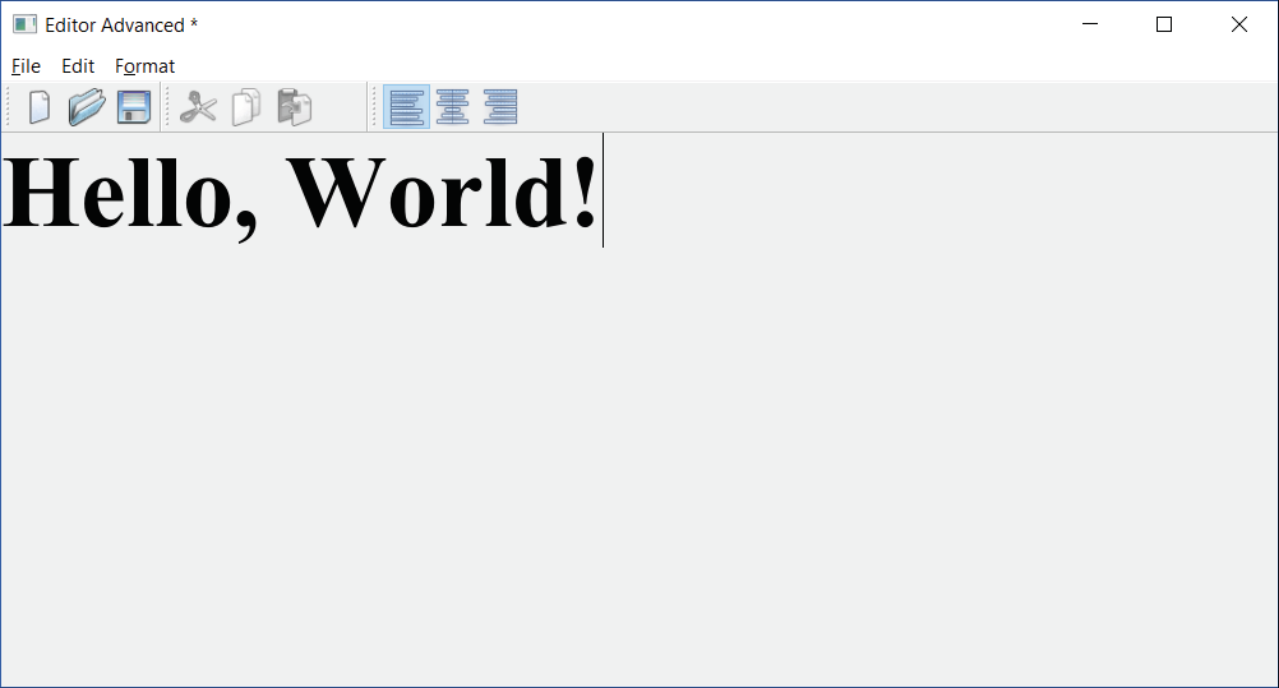
\includegraphics[width=0.9\textwidth]{images/p239_i08.png}\end{center}

\section{小结}

本章我们用 Qt 库开发了三个图形应用——一个模拟时钟、一个画图程序和一个编辑器。时钟显示当前的时、分、秒；画图程序中我们可以绘制直线、矩形和椭圆；编辑器中我们可以输入和编辑文本。

下一章我们将继续完善这些应用，开发更高级的版本。

